\documentclass[12pt]{article}
\usepackage{latexsym} 
\usepackage{graphics} 
\renewcommand{\P}{${\cal{P}}\:$}
\newcommand{\ldot}{.}
\newcommand{\nonterminal}[1]{{<}\mbox{#1}{>}}
\newtheorem{eksempel}{Example}[section]
{\begin{Example}
\mbox{}
\end{Example}}
%%%%%%%%
% \ramme tegner en ramme rundt om noget, dog uden den h|jre
% lodrette streg. Bruges som \framebox, for eksempel:
% 	\ramme{tekst}
% eller \ramme[5cm]{tekst}
% eller \ramme[20mm}[l]{tekst}
\newcommand{\ramme}[3]{\newbox\tempboxa
\newdimen\tempdima
\def\ramme{\@ifnextchar [{\@iramme}{\@yramme}}
\def\@iramme[#1]{\@ifnextchar [{\@xramme[#1]}{\@xramme[#1][x]}}
\def\@yramme#1{\setbox\tempboxa\hbox{~#1}\@ramme}
\def\@xramme[#1][#2]#3{\savebox\tempboxa[#1][#2]{#3}\@ramme}
\long\def\@ramme{\leavevmode\tempdima\fboxrule\advance\tempdima \fboxsep 
  \advance\tempdima \dp\tempboxa \hbox{\lower \tempdima\hbox
  {\vbox{\hrule height \fboxrule
          \hbox{\vrule width \fboxrule \hskip\fboxsep
	    \vbox{\vskip\fboxsep \box\tempboxa\vskip\fboxsep}}
		   \hrule height \fboxrule}}}}}
%%%%%%%%

\parindent 0em
\parskip 1.5ex

\begin{document}
\title{THE BOBS-SYSTEM}
\author{S{\o}ren Henrik Eriksen\thanks{A/S Regnecentralen, Aarhus}\\
Bent B{\ae}k Jensen\thanks{KTAS, K{\o}benhavn}\\
Bent Bruun Kristensen\thanks{Department of Computer Science, Institute of Eletronic Systems,
Aalborg University Center, DK-9000 Aalborg}\\
Ole Lehrmann Madsen}
\date{June 1993}
\maketitle

\begin{abstract}
The BOBS-System is an LALR(1) parser-generator. This paper is a user
manual for the system: Consisting of a general description of the system,
a reference manual, and a summary of parsing terminology. These sections 
can be read without knowledge of parsing theory.

Furthermore, the implementation of the system is described. This is done
by giving references to literature containing descriptions of some of the
algorithms used, and by giving abstract algorithms for other parts of
the system. This section requires that the reader is familiar with LR-parsing.
\end{abstract}
\newpage
\tableofcontents
\newpage


\section*{PREFACE to the Third Edition}
This third edition is identical to the first and second edition
except that some minor errors have been corrected, appendix B has
been added and section 6.1.2 has been replaced by a reference to a
more appropriate source.

\section*{INTRODUCTION}
This paper is a description of a parser-generator system called 
the BOBS-system.

We consider the LR-grammars \cite{3}. 
These are, in ascending order of complexity, LR(0), SLR(k), LALR(k),
L(m)R(k) and LR(k) as defined in \cite{1,2}.

The BOBS-system is an implementation of a parser-generator in the
programming language PASCAL \cite{12} for the SLR(1) and LALR(1)
grammars.

This paper is divided into four parts: part 1 is a general 
description of the system; part 2 is a user manual; in part 3 we
describe the program organization and some algorithms of special
interest; and part 4 contains an introduction to the terminology
which we use. (Readers not familiar with the terminology should 
read this part first.)
\newpage
\part{}
\section{The history of the BOBS-system}
The work was started as an undergraduate project in 1971 under the
guidance of Peter Kornerup. 
The aim of the project was to implement a parser-generator system
for SLR(1)-grammars.
This was fulfilled in March 1972.
The first version was implemented in the earliest version of the
programming language Pascal \cite{6} on a CDC 6400.

A revised version was released in December 1972, and a user manual
\cite{7} appeared in March 1973.
At the same time a short introductory description of the system \cite{8}
was published.

During 1973 the system was extended and modified \cite{9} as a result of
our experiences in using the system.
A new lexical analyser and a new error-recovery method were
implemented.
A new look-ahead algorithm was constructed and implemented,
extending the system to accept LALR(1)-grammars.

During 1974 a new user manual was written.
In October 1974 this manual and system description \cite{8} were
published in \cite{10}.

Since December 1974 a modified version of the system has been
distributed from the University of Texas at Austin by W.F. Burger.
This version is called ``BOBSW -- A Parser Generator'' \cite{11}.

In October 1976 a new modified version of the system was finished.
First of all the parser generator has been translated (more or
less) mechanically into standard Pascal \cite{12}, so that the system is
no longer dependent on the earliest Pascal compiler on the CDC 6400.
Next the parser generator has been extended to handle grammars,
whose grammar rules contain empty productions, without eliminating
such productions.
A new skeleton compiler has been implemented.
This means new lexical, syntax and error-recovery algorithms, and
implementation of a user semantic stack.

\section{Global design of the system}
The system consists of two programs:
\begin{itemize}
\item the parser-generator,
\item the skeleton compiler.
\end{itemize}

\subsection{The parser-generator}
The parser-generator is divided into the following modules:
\begin{itemize}
\item input of the source grammar,
\item grammar checks and grammar transformations,
\item generation of the LALR(1)-tables.
\end{itemize}

\subsubsection{Specification of the source grammar}
The source grammar must be specified in a slightly modified BNF
(Backus Naur Form).

\subsubsection{Grammar checks and grammar transformations}
It has turned out that the implemented grammar checks and
transformations are very useful when designing a grammar for a
language.

The system cannot produce the LALR(1)-tables for an ambiguous
grammar or grammar containing unused nonterminal symbols.

The system performs the following grammar checks:

Test for unused nonterminal symbols:
\begin{itemize}
\item the system checks that every nonterminal except the
goal-symbol appears on both the left and the right side of a
production,
\item the system checks that all nonterminals can be derived from
the goal symbol (the start symbol),
\item the system checks that all nonterminals can derive a string
only containing terminals.
\end{itemize}
Test for ambiguity:
\begin{itemize}
\item the system checks whether any nonterminal is both left and
right recursive. 
If so, the grammar is ambiguous.
\end{itemize}

The system can perform the following transformations on the grammar:
\begin{itemize}
\item If identical productions exist, the grammar can be modified
by removing the unnecessary productions.
\item If any nonterminal can derive the empty string, the grammar
can be modified by eliminating this production.
The modified grammar generates the same language.
\item If there exist single productions, the grammar can be
modified by eliminating all such.
In a single production the left and right side both consist of only
a single nonterminal, and the left side nonterminal does not appear
on the left side of any other production.
\end{itemize}

\subsubsection{Construction of the LALR(1)-tables}
The first step is to construct the LR(0) parse tables and check
whether the grammar is LR(0) or not.
If this fails, the parse tables are extended by means of LALR(1)
lookahead.
If this fails too, the system reports the parse tables in which the
lookahead information is insufficient.
The user must then change the grammar.

If the grammar happens to be LALR(1), the parse tabels are
compressed through a series of various optimizations.

\subsubsection{Output from the parser-generator}
The system delivers the following output:
\begin{itemize}
\item a listing of the source grammar, exactly as the user has
written it. 
Any error according to the input syntax is marked;
\item the results of the above mentioned grammar checks and
transformations:
\item the modified grammar written in BNF.
Each production is assigned a unique number;
\item a description of any parse tables which are not LALR(1);
\item an error message table for use by the user when parsing an
erroneous string;
\item a file containing the parse tables and a file containing the
skeleton compiler (a Pascal program).
\end{itemize}

In addition there exist several other output facilities, mentioned
in Section 4.2.7 but they are of little interest here.

\subsubsection{SLR(1)}
As mentioned in Section 1 the system was originally designed for
SLR(1) grammars.
The possibility of using SLR(1)look-aheads instead of LALR(1) still
exists.

\subsection{The skeleton compiler}
The second part of the system is a Pascal program, which is
delivered as output from the parser-generator.
The unmodified skeleton compiler will check the syntac of an input
string written in the language defined by the source grammar.
However, the user may add semantic actions to the skeleton compiler.

The skeleton compiler is devided into the following modules:
\begin{itemize}
\item the semantic interface
\item the parser part
   \begin{itemize}
   \item lexical analysis
   \item syntax analysis
   \item error recoverly
   \end{itemize}
\end{itemize}

\subsubsection{The semantic interface}
When a reduction is performed, a procedure ``CODE'' is called with
the production (reduction) as a parameter.
The user may then decide what semantic actions to perform.
This is done by writing the body of the procedure ``CODE''.
The user may, of cource, add new procedures and declarations.

\subsubsection{The parser part}
In this part of the program the user does not have to change
anything.

\paragraph{\em 2.2.2.1 {Lexical analysis}}
Characters from the input are read and collected into single
logical items called tokens.
A token corresponds to a terminal symbol of the grammar.

\paragraph{\em 2.2.2.2 {Syntax analysis}}
The syntax analyser uses the parse tables constructed by the
generator to parse the string of tokens delivered from the lexical
analyser.

\paragraph{\em 2.2.2.3 {Error recovery}}
If an error is discovered during parsing, an error recovery
algorithm is called.
The purpose of the recovery algorithm is to mark the symbol causing
the error detection, to recover from the erroneous situation, and
to initialize a continuation of the parsing.

\section{Evaluation}
The system has been used in a variety of different projects. 
A compiler for the language Pascal \cite{6, 13} has been based on the
system.
The Pascal grammar consists of more than 250 productions and the
constructed LALR(1) tables occupy about 1000 60 bit words on a CDC
6400.
Compared with the Z\"{u}rich Pascal Compiler (version 6.\ Sept.\ 72)
the core requirements and execution time are nearly the same.

Inside the department the system has been used for various
compilers and assemblers.
It is also used in a compiler course, in which the students have to
write a small compiler.

At the Danish Data Archive (an institution under the Danish Social
Science Research Council) and at the Institute of Economics,
University of Aarhus, a modified version of the system is used to
implement interactive special purpose languages, which are designed
to ease the use of libraries of statistical programs, the handling
of files and the controlling of data bases. 
This system consists of about 20 grammars each containing from 160
to 250 productions.

As the work has been moving along, new projects have arisen.
Automatic error recovery in LR-parsing has been studied \cite{14}.
Also problems of defining semantics have been studied. 
One project \cite{15} was to extend the system with the Oxford semantics
\cite{16}.
Furthermore the use of attribute grammars in practical translator
writing systems has been studied \cite{17}.

We conclude that the system is usable in practice and that
experience has shown that it is easy to modify grammars to become
LALR(1), even for users who are not familiar with LR-parsing theory.

\part{} 
\section{User Manual}
\subsection{Notation}
The specification of the syntax of input to the parser generator is
given in {\em extended} BNF.
In this notation a set of additional metasymbols is introduced.
These may be used in the specification in the following way:

\begin{description}
\item[\{ \}] clauses enclosed in these parantheses are grouped into a single
clause
\item[*] the clause preceding this symbol may be repeated zero or
more times, 
\item[+] the clause preceding this symbol may be
repeated one or more times, 
\item[?] the clause preceding this
symbol is optional. 
\end{description}

Finally, the metasymbol $::=$ is replaced by the symbol
${\rightarrow}$.

\subsection{Syntax of input to the parser generator}

$\nonterminal{PARSER -- GENERATOR -- SYMBOL} \rightarrow$\\
\hspace*{2cm}
$\begin{array}{l}
 \{\nonterminal{OPTIONLIST}\} ?\\
 \{\nonterminal{METASYMBOL -- DEFINITION}\} ?\\
 \{\nonterminal{TERMINAL -- DEFINITION}\} \\
 \{\nonterminal{STRINGCH -- DEFINITION}\} ?\\
 \{\nonterminal{GOALSYMBOL -- DEFINITION}\} ?\\
 \{\nonterminal{COMMENT -- DEFINITION}\} ?\\
 \{\nonterminal{GRAMMAR -- RULE} \mid \nonterminal{METASYMBOL --
DEFINITION}\}^{\ast}\\
 \nonterminal{ENDCH}
\end{array}$

\subsubsection{Metasymbols}
\begin{tabbing}
\=$\nonterminal{METASYMBOL-DEFINITION} \rightarrow$\\
\> METASYMBOLS $\nonterminal{M1} \nonterminal{M2} \nonterminal{M3} \nonterminal{M4}$\\ 
\>$\nonterminal{M1} \rightarrow \mbox{M1} = \nonterminal{CH}$\\
\>$\nonterminal{M2} \rightarrow \mbox{M2} = \nonterminal{CH}$\\
\>$\nonterminal{M3} \rightarrow \mbox{M3} = \nonterminal{CH}$\\
\>$\nonterminal{M4} \rightarrow \mbox{M4} = \nonterminal{CH}$\\
\end{tabbing}
$\nonterminal{CR}$ is any
character other than a letter, a digit or a space.

The metasymbols must be different.
The correspondence to the use in BNF is:

\begin{tabbing}
\hspace*{2cm}\=M1xx\=works asxx \= $::=$ \kill
\>M1\>works as \> $::=$\\
\>M2\>works as \> $|$\\
\>M3\>works as \> ${<}$ and ${>}$\\
\>M4\>indicates the termination of a sequence of alternatives \\
\>  \>in a grammar rule.
\end{tabbing}

Default metasymbols are:
\begin{center}
M1$==$, M2$=/$, M3$=<$, and M4$=;$
\end{center}

In the following M1, M2, M3, and M4 denote the current metasymbols.

\subsubsection{Terminals}
$\nonterminal{TERMINAL -- DEFINITION} \rightarrow
\nonterminal{TERMINAL}^{\ast} \ \ \ \mbox{M4}$

All terminal symbols used in the grammar must be listed.
A terminal symbol consists of at most 10 character.
The characters set has been divided into two groups:

\begin{itemize}
\item letter and digits
\item all other characters except space
\end{itemize}

All the characters forming a terminal must belong to the same set of the above
groups.
Terminals consisting of symbols from group 1 must start with a letter.\\
No terminal may contain the current M4.\\
The terminal symbols in the list must be delimited by spaces and/or
end-of-lines.

The following terminals have a special interpretation.
If they are used in the grammar, they must be listed among the 
other terminals.
\begin{tabbing}
EMPTY \ \ \ \ \= denotes the empty string.\\
NAME          \> denotes an identifier. (A sequence of letters and digits with the\\
              \> first symbol being a letter.)\\
KONST         \> denotes a constant. (A sequence of letters and digits with the \\
              \> first symbol being a digit.)\\
STRING        \> denotes a string constant. (A string is a sequence of characters\\
              \> surrounded by a string-escape-character. If the string-escape-\\
              \> character is used in the string, it must be written two times per\\
              \> occurrence.\\
ERROR         \> denotes an error symbol. The use of the error-symbol is\\
              \> explained in Section 5.3.
\end{tabbing}

\subsubsection{Stringch}
$\nonterminal{STRINGCH -- DEFINITION} \rightarrow \mbox{STRINGCH} =
\nonterminal{CH} \ \ \ \mbox{M4}$

Defines the string-escape-character to be the character $<$CH$>$. It
must not be contained in any other terminal symbol. No default value
exists.

\subsubsection{Grammar-rule}
$\begin{array}{lll}
\nonterminal{GRAMMAR - RULES} &\rightarrow &
\nonterminal{NONTERMINAL} \mbox{M1} \nonterminal{ALTERNATIVE}\\
&& \{\mbox{M2} \nonterminal{ALTERNATIVE}\}^* \mbox{M4}\\
\nonterminal{ALTERNATIVE} & \rightarrow &
\{\nonterminal{NONTERMINAL} \mid \nonterminal{TERMINAL}\}^+\\
\nonterminal{NONTERMINAL} &\rightarrow & \mbox{M3 a sequence of
characters M3}
\end{array}$

The sequence of characters must not contain the current M3.
Spaces are skipped.
A nonterminal may consist of up to 30 characters.
Terminals and nonterminals in a rule must be separated by spaces or end of
lines.

If EMPTY is used it must be the only symbol in that alternative.

The terminals in a grammar rule must not contain any of the metasymbols
currently defined.
If they have to, the metasymbols must be redefined.
It is not necessary for all alternatives to the same lefthandside of a grammar
rule to be defined at the same time, they may be defined later.

\subsubsection{Goalsymbol}
\begin{tabbing}
$\nonterminal{GOALSYMBOL -- DEFINITION}$\= $\rightarrow \nonterminal{GOALSYMBOL}$ \\ 
                                        \> $= \nonterminal{NONTERMINAL} \ \ \ \mbox{M4}$
\end{tabbing}
Defines the nonterminal to be the goalsymbol of the grammar.
If this command is not present, the first nonterminal met among the grammar
rules is assumed to be the goalsymbol.

The parser generator always adds the following grammar
rule (production no. 0):

\[
\nonterminal{BOBS -- GOAL} \rightarrow
\nonterminal{GOALSYMBOL} \mbox{END--OF--FILE}
\]

\subsubsection{Endcharacter}
$\nonterminal{ENDCH} \rightarrow \mbox{M4}$

The input to the parser generator must be terminated by the currently defined
M4.

\subsubsection{Comment}
\begin{tabbing}
$\nonterminal{COMMENT} \rightarrow \nonterminal{COMMENT}$ $=$ \= $\nonterminal{COMMENT -- BEGIN} \ \ \ \mbox{M4}$\\
                                                              \> $\nonterminal{COMMENT -- END} \ \ \ \mbox{M4}$\\
$\nonterminal{COMMENT -- BEGIN} \rightarrow \nonterminal{TERMINAL}$\\
$\nonterminal{COMMENT -- END} \rightarrow
\;\mbox{a sequence of characters}$\\
\end{tabbing}
$\nonterminal{TERMINAL} \;\mbox{must be defined in the}
\nonterminal{TERMINAL -- DEFINITION}$ (4.2.2)
The sequence of characters of $\nonterminal{COMMENT -- END}$ must
not include the current M4. Spaces are skipped.

In the input string to be parsed the following is considered to 
be a comment:
\begin{tabbing}
$\nonterminal{COMMENT -- BEGIN}$ any sequence of characters \\
 \ \ \ \ \ \ \ \= (except \= $\nonterminal{COMMENT -- END}$)\\
               \>         \> $\nonterminal{COMMENT -- END}$
\end{tabbing}
See also Section 5.1.

\subsubsection{Options}

\begin{tabular}{lll}
$\nonterminal{OPTIONLIST}$ & $\rightarrow$ & $\nonterminal{OPTION}
(\nonterminal{OPTION -- NUMBER}$\\ & & $\{, \nonterminal{OPTION --
NUMBER}\}^*)$ 
\end{tabular}


$\nonterminal{OPTION -- NUMBER}$ is an integer.
Most of the options are for test purposes only, and some may cause an error in
the generated parser.
The options are implemented as switches, which means that 
if the same number is used twice, the option is returned to the
original position.

For most users, the rest of this section is of no interest, and 
may be skipped.

The following numbers are valid:


\begin{tabbing}
1 \ \ \ \ \ \ \ \= The internal representations of the terminal symbols are printed.\\
2               \> The LR(0) tables are printed.\\
3               \> The terminal symbols may be collected in sets where all terminals\\ 
                \> in such a set are given the same internal value. \\
                \> Let T1, T2, $\ldot$, TN be terminals.\\
                \> If in the list of terminals (4.2.2) you write:\\
                \> \hspace*{2cm}T1 T2 M1 T3 M1 $\ldot$ M1 TN M1\\
                \> then T1, T2, $\ldot$, TN are all given the same internal value.\\
                \> There must be exactly one space between a terminal and M1.\\
                \>In all outputs, T1, T2, $\ldot$, TN-1 will appear as TN.\\
4               \> The lenght of the terminal symbols may be greater than 10 characters.\\
                \>All characters are significant but only the 10 first appear in output.\\
5               \> The terminal symbols may consist of characters from both character\\
                \> groups (see chapter 4.2.2).\\
                \> The terminal symbols must be separated by blanks or an end-of-line.\\
                \> (The lexical analyser in the skeleton compiler must be modified for these\\
                \> terminals.)\\
6               \> The internal values of the nonterminal symbols are printed.\\
7               \> The SLR(1) lookahead symbols for each nonterminal are printed.\\
                \> (Caution: option 27 must be used.)\\
12              \> The inadequate LR(0) tables are printed.\\
14              \> The internal form of the LR(0) tables is printed.\\
15              \> The internal form of the LR(0) tables and the generated lookback\\
                \> tables are printed.\\
16              \> The internal array ``PROD'' is printed.\\
17              \> The internal array ``TILSTAND'' is printed.\\
18              \> The terminal heads and tails which a nonterminal can\\
                \> produce are printed.\\
19              \> Test information of ``VHRECURS'' is printed.\\
20              \> The bit matrix of the grammar is printed.\\
21              \> Test information of ``LOOKBACK'' is printed.\\
22              \> The largest lookahead set is not removed from a lookahead table.\\
                \>(The table is treated like a lookahead--error table.)\\
23              \> The internal form of the productions is printed before the grammar is\\
                \> modified.\\
24              \> The internal form of the productions is printed after the grammar is\\
                \> modified.\\
25              \> No attempt is made to test for left and right recursion.\\
27              \> The grammar is treated as an SLR(1) grammar instead of an LALR(1)\\
                \> grammar. \\
                \> In this case one has to use option 31 too.\\
28              \> No attempt is made to remove the single productions.\\
29              \> Tables which have the same tail are not folded together.\\
30              \> The LR(0) items are printed in a readable form.\\
31              \> The empty string is eliminated from the grammar.\\
32              \> Files PARSIN and PARSOUT (see appendix A) are ignored.\\
                \> Only parse tables are produced (on file TABLES).\\
\end{tabbing}

\subsection{Constants}
The following constants define the maximum sizes of the data structures in the
parser--generator.

Most of the constants are totally internal to the program and should only be
changed with care.

\begin{description}
\item[CONST 1] \ Maximum number of productions.
\item[CONST 2] \ Maximum number of terminal and nonterminal symbols.
\item[CONST 3] \ Maximum size of array FCQ.
\item[CONST 4] \ Maximum size of array RHS.
\item[CONST 5] \ Maximum number of elements in a basis set of an LR(0) table.
\item[CONST 7] \ Maximum size of final parse tables.
\item[CONST 8] \ Maximum number of lookahead elements for a nonterminal.
\item[CONST 9] \ Maximum size of aray STACK in procedure LR0.
\item[CONST 10] Maximum number of parse tables.
\item[CONST 11] Maximum number of nonterminals.
\item[CONST 12] Maximum number of terminals.
\item[CONST 13] Equal CONST2DIV (SETMAX=1) = 1  \footnote{CONST
SETMAX = 58 in the CDC version.}
\item[CONST 14] Maximum size of a parse table.
\item[CONST 16] Maximum number of options.
\item[CONST 18] Maximum number of options.
\end{description}

\subsection{Error messages}
Two types of error messages can occur:
\begin{itemize}
\item system errors
\item errors according to the grammar.
\end{itemize}

\subsubsection{System errors}
One of the data structures in the parser generator has caused an error.
The appropriate constant must be changed in the parser generator.

\subsubsection{Errors according to the input grammar}
There might be errors:
\begin{itemize}
\item in input to the parser generator,
\item according to the grammar checks and grammar transformations,
\item in the parse tables, which are not LALR(1).
\end{itemize}

\section{The Skeleton Compiler}
When using the parser--generator, the Skeleton--compiler must reside on file
PARSIN.
The parser--generator then delivers the Skeleton--compiler with initialized
constants on the file PARSOUT.
The parse tables associated with the user's grammar are delivered on the file
TABLES.
It would have been more handy to incorporate the parse tables in the
Skeleton--compiler as a set of initializations, but this is however not
possible in Standard PASCAL.

The Skeleton--compiler consists of
\begin{itemize}
\item PROCEDURE PARSER,
\item PROCEDURE CODE, and
\item some global declarations.
\end{itemize}

The procedure PARSER is the major part of the Skeleton--compiler.
It consists of procedures for doing:
\begin{itemize}
\item Lexical analysis,
\item Context--free syntax analysis (parsing), and
\item Error recovery.
\end{itemize}

We shall not discuss these procedures her, but the reader is referred to
section 5.1 for a specification of how the input string to the lexical analyser
must look.
The use of the special tokens NAME, KONST, and STRING is
explained in section 5.2.2.
Error recovery is treated in section 5.3.

The procedure CODE is an almost empty procedure which has to be written by the
user.
CODE is called from the parser each time a reduction is performed  during the
parsing of a string.
In this way CODE will act as an interface between the parser and the semantic
part of a compiler based on the Skeleton--compiler.

Among the global declarations is a stack which may be used by the user (see
section 5.2.3).

\subsection{Input/Output of the Skeleton--compiler}
Input to the Skeleton--compiler:
\begin{itemize}
\item On file INPUT: a string in the language generated by the grammar.
Terminals in this string must be separated by spaces and/or end-of-lines.
However two terminals may be concatenated if they are not in the same group of
characters (see section 4.2.2.).
Terminals from group 2 may be concatenated if the concatenation does not
together form the head of another terminal.
Spaces and/or end-of-lines are only allowed as separators between terminals and
are considered as blind characters.
A comment may appear between any two terminals.
It may be necessary to surround $\nonterminal{COMMENT--BEGIN}$ by
spaces in order to avoid that $\nonterminal{COMMENT--BEGIN}$
concatenated with the preceeding terminal and/or the beginning of a
comment forms the head of some terminal.
\item On file TABLES: the parse tables of the grammar. 
\end{itemize}
Output from the Skeleton--compiler (on file OUTPUT):
\begin{itemize}
\item A listing of the input string.
Possible syntax errors in the string are marked (see section 5.3).
\item A snapshot of the parse.
Contains a general print-out of the steps in the parse of the actual input
string.
It is intended as an aid to the user and may be removed.
\end{itemize}

\subsection{Adding Semantics}
As mentioned, the procedure CODE is called from the parser each time a
reduction is performed.
CODE has as parameter the number of the applied production.
The productions are numbered according to the listing produced by the
parser-generator (see section 2.1.4).

Inside CODE, an appropriate action must be taken for each production in the
grammar.

Besides filling out the body of CODE, the user is free to add new global
declarations (procedures, variables, etc.).

As the parsing method is LR, the reductions will be performed in the order of a
so-called {\bf right-parse}.
It is fundamental for using the BOBS-system, that the notion of a right-parse
is understood.
A definition of a right-parse is given in part IV.
The snapshot of the parse may be an aid in understanding the order of the
reductions.

\subsubsection{Using NAME, KONST, and STRING}
If the symbols NAME, KONST, and STRING are used on the right
side of a production, then the user can get the string of characters
actually comprising the NAME, KONST, or STRING.
This is done by means of:

\begin{tabbing}
\hspace{1cm} \= proc \= \kill
         \> {\bf PROCEDURE} GETSTRING (NO. INTEGER;\\
          \>  \> {\bf VAR} STR: STRING {\bf VAR} LENGTH:
INTEGER); 
\end{tabbing}

where STRING = {\bf PACKED ARRAY}[1..STRINGMAX] 
{\bf OF} CHAR;

Suppose CODE is called with the number of production

\[x_0 \rightarrow x_1 {\ldots} x_i {\ldots} x_n\]

If $x_i$ is NAME, KONST, or STRING, then

\[
\mbox{GETSTRING} (i,S,L)\; \mbox{or GETSTRING}(-(n-i+1),S,L)
\]
will deliver the corresponding string og characters in S[1],
$\ldots$,S[L].\\
$(S[L+1],\ldots,S[STRINGMAX]$ are undefined.)

If $X_i$ is neither NAME, KONST, nor STRING, then the call of
GETSTRING will deliver an arbitrary string (usually the empty
string).

\subsubsection{Using the Semantic Stack}
In order fully to understand this section, the user must have s
ome knowledge of
how an LR-parser works.
The essence of this is given in part IV.

A stack is a useful tool when implementing the semantics of a 
language, especially if the language contains constructions, which
may be nested. For this reason, the Skeleton--compiler contains a
stack which operates in parallel with the parse stack:


\hspace*{1cm} ATTSTACK: {\bf ARRAY}[STACKINX] {\bf OF} ATTRIBUTES;\\
\hspace*{1cm} ATTRIBUTES = {\bf RECORD} \ldots {\bf END};


The user may define fields in record ATTRIBUTES.
A field in this record will be called an attribute, and the entire
record an attribute record.

During parsing each symbol on the parse stack has a corresponding
attribute record on ATTSTACK.
When a reduction is performed and CODE is called, the topmost
elements of ATTSTACK correspond to the symbols on the right side of
the applied production.

In CODE the values of these attribute records of the right-side
symbols may then be used in the semantic action.
The semantic action of the applied production should define the
value of the attribute record of the left-side symbol.

In order to access the relevant attribute records, CODE is supplied
with two parameters:

\hspace*{1cm} 
OLDTOP, NEWTOP: STACKINX;

OLDTOP is the index in ATTSTACK of the topmost element before
the reduction (at entry to CODE). 
NEWTOP is the index of the topmost element after the reduction is
performed (after exit from CODE).
If the right side of the applied production has the length $N$, the
OLDTOP = NEWTOP+N-1.
NEWTOP is furthermore the index of the attribute record which will
correspond to the left side of the applied production.
I.e.\ the attribute record of the first symbol on the right side
will be used (after modifications done by the user) as the
attribute record of the left side.

Let the applied production be
\[
A \rightarrow x_1 x_2 {\ldots} x_n
\]

At entry to CODE the situation is: See Figure 1.

\begin{figure}[h]
\centerline{\includegraphics{PB71.ATTSTACK.xfig.eps}}
\caption{ATTSTACK}
\end{figure}

$\hat{x}_i (i = 1,2 \ldots, n)$ denotes the attribute record of
$x_i$. 
Then 
\begin{quotation}
\begin{tabbing}
 \ \= ATTSTACK[NEWTOP+i-1] or\\
   \> ATTSTACK[OLDTOP-n+i]
\end{tabbing}
\end{quotation}
is the attribute record of $x_i$. If $i = 1$, then
\begin{quotation}
\begin{tabbing}
 \ \= ATTSTACK[NEWTOP] or\\
   \> ATTSTACK[OLDTOP-n+1]
\end{tabbing}
\end{quotation}
is also the attribute record of $A$.

Lastly we would like to make some remarks concerning some relevant
theoretical models for specifying semantics.

Attribute grammars \cite{21}, Syntax Directed Translation Schemes \cite{20},
and Attributed Translations \cite{22} may all be implemented by using
the ATT STACK.

However only certain restricted classes of these models are
efficient to implement.

The following models should be straightforward to implement:
\begin{itemize}
\item attribute grammars using only synthesized attributes \cite{21}
\item postfix simple syntax directed translation schemes \cite{20}
\item generalized syntax directed translation schemes with
translation elements which are not only string--valued and with the
string translation grammars being postfix and simple \cite{20}
\item attributed polish translation grammars using only synthesized
attributes \cite{22}.
\end{itemize}

The latter two models are in principle identical and are a
combination of the first two alternatives.
Informally the semantic action of a production in these models is:

\begin{itemize}
\item on basis of the attribute records of the right-side symbols
do:
   \begin{itemize}
     \item output some symbols,
     \item define the value of the attribute record of the
      left-side symbol.
    \end{itemize}
\end{itemize}

Translation schemes which are not postfix (polish) and/or simple,
may also be implemented.
This requires that the attribute record contains pointers to the
translation elements, which have to be built in the form of a tree;
for a further study see Aho \& Ullmann \~cite[chapter 9]{20}.

The implementation of inherited attributes or translations is
inefficient in the BOBS--system.
The only way to do it is to build the entire syntax tree and then
perform the evaluation of the attributes.

However in practice it suffices to keep the inherited (or context)
information (e.g. \ a symbol table) in global variables, and update
this information appropriately.

We conclude this section by advocating the following model for
specifying the semantics:
\begin{itemize}
\item make the grammar postfix, i.e. \ code only has to be outputted
at the time of a reduction,
\item define a suitable set of (synthesized) attributes for each
nonterminal,
\item define a set of global variables for collecting declarative
information (i.e. \ a symbol table).
\end{itemize}

\subsection{Error Recovery}
The parser will take error action if the user specifies a string
which is not in the language generated by the grammar.
The error will be detected at the earliest possible point: that is,
the part of the input string which has been read up till this point
will constitute a correct prefix of some string in the language
where the next symbol read is not a valid continuation of the
already read part.
The symbol at which an error is detected will be marked with a
$\uparrow$ and a number. 
The number refers to the error message table which is part of the
output from the parser generator (see 2.1.4).
The number indicates in the error message table a set of terminals
that would have been valid continuations at that point of the input
string.
Note that the set of terminals does not always contain all valid
continuations.

When an error has been detected, the parser tries to continue
parsing.
This can be done in the following way:

Let $A \rightarrow \mathbf{\alpha}$ be a production.
Assume that an error happens in a part of the input which later may
reduce to $\mathbf{\alpha}$ and then to $A$.
We then have recognized part of $\mathbf{\alpha}$. Let $\mathbf{\alpha} = \mathbf{\alpha'\;
\alpha''}$ where $\mathbf{\alpha'}$ is recognized ($\mathbf{\alpha'}$ may be empty).
The parse stack then contains $\varphi \;\mathbf{\alpha'} \;\delta$, for
some  $\varphi$ and $\delta$.
 This means that $\delta$ and some of
the input symbols (if there were no errors) could reduce to
$\mathbf{\alpha''}$ and then $\mathbf{\alpha'}\;\mathbf{\alpha''}$ to $A$.
A possible way of recovering would be to assume that $\mathbf{\alpha''}$ has
been recognized.
This can approximately be done by deleting $\delta$ from the stack
and skip symbols on input until meeting one which may follow
$\alpha''$.

In practice the parser is simultaneously looking for several right
sides of different productions which may reduce to different
nonterminals.
For this reason the user must specify the so--called error
productions in order to indicate the nonterminals that the recovery
algorithm should try to reduce to.

An error production has the form
\[
A \rightarrow \mathbf{\alpha} \;\mbox{error} \; \beta
\]
where error is a special terminal (se Section 4.2.2), and $\mathbf{\alpha}$
and $\beta$ are (possibly empty strings) of nonterminals and
terminals.

Let $A \rightarrow \mathbf{\alpha} \gamma$ be another A-production.
Let the stack at a given time during the parse contain $\varphi\;
\mathbf{\alpha}\; \delta$ for some $\varphi$ and $\delta$.
Assume that $\delta$ and some terminal string $x$ may reduce
to $\gamma$ and then $\mathbf{\alpha}\gamma$ to A.
Assume that $x$ is a prefix of some terminal string which is a
valid continuation on input with the above stack.

Suppose that an error appears in this situation, i.e.\ the next
input symbol is not a valid continuation.
The parser will then replace $\gamma$ by error $\beta$ in
the following way:
\begin{itemize}
\item $\delta$ is deleted from the stack
\item the symbol error is read
\item input symbols are skipped until meeting one which may begin
$\beta$.\\
If $\beta$ is the impty string one skips to a symbol which
may follow $A$ after $\mathbf{\alpha}$ error is reduced to $A$.
\end{itemize}

As $A \rightarrow \mathbf{\alpha}$ error $\beta$ is a usual production.
CODE will be called with the number of the error production.
In this way the user is informed when syntax errors appear.

In general more than one error production may be applicable.
In this case the parser will choose the one which gives rise to
fewest skips on input.

As error productions are normal productions they may give rise to
LR--conflicts which of course must be eliminated.

In order to obtain a successful recovery the user must specify a
reasonable set of error productions.
All parts of the grammar shold be covered as should different
levels in nested constructions.

In general, an error production $A \rightarrow \mathbf{\alpha}$ error
$\beta$ only makes sense if $\mathbf{\alpha}$ is a prefix of some other
production with $A$ as leftside, and $\beta$ should in a similar
way be a postfix.
It is often sufficient to let $\mathbf{\alpha}$ and/or $\beta$ be the empty
string.

\subsection{Examples}
Here is an example of using the skeleton--compiler and tables as
produced by the parser generator in example 4.1.

\begin{eksempel}
\mbox{}
\begin{tabbing}
\texttt{($\#$BOBS EXAMPLE $\#$)}\\
\texttt{DECLARE}\ \ \= \texttt{A,B:}\\
                    \> \texttt{A$:=$1; B$:=$0;}\\
                    \> \texttt{WHILE} \=  \texttt{A $<>$ ($\#$THIS IS A COMMENT $\#$)} \ \ \texttt{$10$}\\
                    \> \texttt{DO}    \> \ \\
                    \>                \> \texttt{A $:=$ A $+ 1$; B $:=$ B $+ +$ A;}\\
                    \> \texttt{OD};\\
                    \> \texttt{WRITE(B).}\\
\\
\texttt{ ($\#$BOBS EXAMPLE $\#$)}\\
\texttt{DECLARE} \= \texttt{A,B:}\\
                 \> \texttt{A$:=$1; B$:=$0;}\\
                 \> \texttt{WHILE} \= \texttt{A $<>$ ($\#$THIS IS A COMMENT$\#$)} \ \ \texttt{$10$}\\
                 \> \texttt{DO}\\
                 \>                \> \texttt{A $:=$ A $+ 1$; B $:=$ B $+ +$} \= \texttt{A;}\\
                 \>                \>                                         \>\texttt{$\hat{} \ 4$}\\
                 \> \texttt{OD};\\
                 \> \texttt{WRITE(B).}\\
\end{tabbing}
\mbox{}
\texttt{SNAPSHOT:}
\begin{tabbing}
\texttt{LEXICAL:} \ \ \ \ \ \=($\#$ \ \ \ \ \ \ \ \= $\mid$ \ \= \texttt{LEXICAL : DO} \ \ \ \ \ \= $\mid$ \ \= \texttt{PRODUCTION :} $5$\\
\texttt{LEXICAL:}       \>\texttt{DECLARE}    \> $\mid$   \> \texttt{PRODUCTION :} 11        \> $\mid$   \> \texttt{LEXICAL : WRITE}\\
\texttt{LEXICAL:}       \>\texttt{A}          \> $\mid$   \>  \ \ \texttt{SYMB1} 10          \> $\mid$   \> \texttt{LEXICAL : (}\\
\texttt{LEXICAL:}       \>\texttt{,}          \> $\mid$   \> \texttt{PRODUKTION :} 41        \> $\mid$   \> \texttt{LEXICAL : B}\\
\texttt{PRODUKTION:}    \>9                   \> $\mid$   \> \texttt{PRODUKTION :} 37        \> $\mid$   \> \texttt{LEXICAL : )}\\ 
 \ \ \texttt{SYMB1 \ A} \>                    \> $\mid$   \> \texttt{PRODUKTION :} 31        \> $\mid$   \> \ \ \texttt{SYMB1 B )}\\  
\texttt{PRODUCTION:}     \>8                   \> $\mid$   \> \texttt{PRODUKTION :} 25        \> $\mid$   \> \texttt{PRODUCTION :} 40\\
\texttt{LEXICAL:}       \>\texttt{B}          \> $\mid$   \> \texttt{LEXICAL : A}            \> $\mid$   \> \texttt{PRODUKTION :} 37\\
\texttt{LEXICAL:}       \>;                   \> $\mid$   \> \texttt{LEXICAL : } $:=$        \> $\mid$   \> \texttt{PRODUKTION :} 31\\
\texttt{PRODUKTION:}    \>9                   \> $\mid$   \> \texttt{PRODUKTION :} 23        \> $\mid$   \> \texttt{PRODUKTION :} 26\\ 
 \ \ \texttt{SYMB1 \ B} \>                    \> $\mid$   \> \ \ \texttt{SYMB1 A}            \> $\mid$   \> \texttt{PRODUKTION :} 28\\ 
\texttt{PRODUKTION:}    \>7                   \> $\mid$   \> \texttt{LEXICAL : A}            \> $\mid$   \> \texttt{LEXICAL : } $\ldot$\\ 
\texttt{LEXICAL:}       \>\texttt{A}          \> $\mid$   \> \texttt{LEXICAL :} $+$          \> $\mid$   \> \texttt{PRODUKTION :} 20\\
\texttt{PRODUCTION:}     \>3                   \> $\mid$   \> \texttt{PRODUKTION :} 23        \> $\mid$   \> \texttt{PRODUCTION :} 5\\
\texttt{LEXICAL:}       \>$:=$                \> $\mid$   \>  \ \ \texttt{SYMB1 A}           \> $\mid$   \> \texttt{LEXICAL : }\\
\texttt{PRODUCTION:}     \>23                  \> $\mid$   \> \texttt{PRODUKTION :} 40        \> $\mid$   \> \texttt{PRODUCTION :} 1\\
 \ \ \texttt{SYMB1 \ A} \>                    \> $\mid$   \> \texttt{PRODUKTION :} 37        \> $\mid$   \> \texttt{LEXICAL :}\\  
\texttt{LEXICAL:}       \>1                   \> $\mid$   \> \texttt{PRODUCTION :} 31        \> $\mid$\\
\texttt{LEXICAL:}       \>;                   \> $\mid$   \> \texttt{LEXICAL :} 1            \> $\mid$\\
\texttt{PRODUCTION:}     \>11                  \> $\mid$   \> \texttt{PRODUKTION :} 34        \> $\mid$\\
 \ \ \texttt{SYMB1 \ 1} \>                    \> $\mid$   \> \texttt{LEXICAL : ;}            \> $\mid$\\  
\texttt{PRODUCTION:}     \>41                  \> $\mid$   \> \texttt{PRODUKTION :} 11        \> $\mid$\\
\texttt{PRODUCTION:}     \>37                  \> $\mid$   \>  \ \ \texttt{SYMB1 1}           \> $\mid$\\
\texttt{PRODUCTION:}     \>31                  \> $\mid$   \> \texttt{PRODUKTION :} 41        \> $\mid$\\
\texttt{PRODUCTION:}     \>26                  \> $\mid$   \> \texttt{PRODUKTION :} 37        \> $\mid$\\
\texttt{PRODUCTION:}     \>15                  \> $\mid$   \> \texttt{PRODUKTION :} 30        \> $\mid$\\
\texttt{PRODUCTION:}     \>6                   \> $\mid$   \> \texttt{PRODUKTION :} 26        \> $\mid$\\
\texttt{LEXICAL:}       \>\texttt{B}          \> $\mid$   \> \texttt{PRODUKTION :} 15        \> $\mid$\\
\texttt{LEXICAL:}       \>$:=$                \> $\mid$   \> \texttt{PRODUKTION :} 6         \> $\mid$\\
\texttt{PRODUCTION:}     \>23                  \> $\mid$   \> \texttt{LEXICAL : B}            \> $\mid$\\
 \ \ \texttt{SYMB1 \ B} \>                    \> $\mid$   \> \texttt{LEXICAL : } $:=$        \> $\mid$\\  
\texttt{LEXICAL:}       \>0                   \> $\mid$   \> \texttt{PRODUCTION :} 23        \> $\mid$\\
\texttt{LEXICAL:}       \>;                   \> $\mid$   \>  \ \ \texttt{SYMB1 B}\\
\texttt{PRODUCTION:}     \>11                  \> $\mid$   \> \texttt{LEXICAL : B}\\
 \ \ \texttt{SYMB1 \ 0} \>                    \> $\mid$   \> \texttt{LEXICAL :} $+$\\  
\texttt{PRODUCTION:}     \>41                  \> $\mid$   \> \texttt{PRODUKTION :} 23\\ 
\texttt{PRODUCTION:}     \>37                  \> $\mid$   \>  \ \ \texttt{SYMB1 B}\\
\texttt{PRODUCTION:}     \>31                  \> $\mid$   \> \texttt{PRODUKTION :} 40\\ 
\texttt{PRODUCTION:}     \>26                  \> $\mid$   \> \texttt{PRODUKTION :} 37\\ 
\texttt{PRODUCTION:}     \>15                  \> $\mid$   \> \texttt{PRODUKTION :} 31\\ 
\texttt{PRODUCTION:}     \>5                   \> $\mid$   \> \texttt{LEXICAL :} $+$\\
\texttt{LEXICAL:}       \>\texttt{WHILE}      \> $\mid$   \> \texttt{PRODUCTION :} 34\\
\texttt{LEXICAL:}       \>\texttt{A}          \> $\mid$   \> \texttt{LEXICAL : A} $<$\texttt{---SYNTAKSERROR} \texttt{$<$---SKIPPED}\\
\texttt{LEXICAL:}       \>$<>$                \> $\mid$   \> \texttt{LEXICAL : ;}\\
\texttt{PRODUCTION:}     \>23                  \> $\mid$   \> \texttt{PRODUKTION :} 27\\ 
 \ \ \texttt{SYMB1 \ A} \>                    \> $\mid$   \> \texttt{PRODUKTION :} 15\\  
\texttt{PRODUCTION:}     \>40                  \> $\mid$   \> \texttt{PRODUKTION :} 5\\ 
\texttt{PRODUCTION:}     \>37                  \> $\mid$   \> \texttt{LEXICAL : OD} \\ 
\texttt{PRODUCTION:}     \>31                  \> $\mid$   \> \texttt{PRODUKTION :} 14\\ 
\texttt{LEXICAL:}       \>($\#$               \> $\mid$   \> \texttt{PRODUKTION :} 5\\
\texttt{LEXICAL:}       \>10                  \> $\mid$   \> \texttt{LEXICAL : ;}\\
\texttt{PRODUCTION:}     \>33                  \> $\mid$   \> \texttt{PRODUKTION :} 17\\   
\end{tabbing}
\end{eksempel}
\subsubsection*{Example 5.2}
This example shows how a simple translation can be implemented.
We define a small language with simple control structures,
assignments, expressions and Algol like blocks with dclaration of
variables.
A variable must be declared before it is used and double
declarations in a block may not appear.
All language constructs are translated into an equivalent one.
The major transformations are : variables are added the nesting
depth of the block in which they are declared, expressions are
transformed to postfix polish, the control structures are extended
with line numbers indicating possible jumps.
The grammar has been transformed in order to make the translation
polish.

The following pages contain
\begin{itemize}
\item a listing of the grammar,
\item all global label, const, type, and var declarations of the
skeleton compiler, including the ones added for the semantic
example,
\item the part of the procedure CODE which has been added for the
semantic example, and
\item an example of a translation.
\end{itemize}
\begin{eksempel}
\mbox{}
\begin{tabbing}
$\ast\ast\ast\ast\ast\ast\ast\ast\ast\ast\ast\ast\ast\ast$ \texttt{THE GRAMMAR} $\ast\ast\ast\ast\ast\ast\ast\ast\ast\ast\ast\ast\ast\ast$\\
\ \ 1 \ \ \ \ \ \= $<$\texttt{PROGRAM}$> ::= <$\texttt{START}$> \ <$\texttt{BLOCK}$>$ $\cdot$\\
\ \ 2           \> $<$\texttt{START}$> ::=$ \texttt{EMPTY}\\  
\ \ 3           \> $<$\texttt{BLOCK}$> ::= <$\texttt{BLOCKDEC}$>$ \ $<$\texttt{STATEMENTSEQ}$>$ \texttt{END}\\
\ \ 4           \> $<$\texttt{BLOCKDEC}$> ::= <$\texttt{BEGIN}$>$ \ $<$\texttt{DECLARATION}$>$\\
\ \ 5           \> $<$\texttt{STATEMENTSEQ}$> ::=$\= $<$\texttt{STATEMETNSEQ}$>$ \texttt{;} $<$\texttt{STATEMENT}$>$\\
\ \ 6           \>                                \> $<$ \texttt{STATEMENT}$>$\\  
\ \ 7           \> $<$\texttt{BEGIN}$> ::=$ \texttt{BEGIN}\\
\ \ 8           \> $<$\texttt{DECLARATION}$> ::=$\= $ <$\texttt{DECID} ; \texttt{DECLARATION}$>$\\
\ \ 9           \>                                \> \texttt{EMPTY}\\
\ 10            \> $<$\texttt{DECID}$> ::= <$\texttt{DECLARE NAME}\\
\ 11            \> $<$\texttt{STATEMENT}$> ::=$\= $<$\texttt{IFTHEN}$> <$\texttt{STATEMENTSEQ}$>$ \texttt{FI}\\
\ 12            \>                             \> $/ <$\texttt{WHILECLAUSE}$> \ <$\texttt{STATEMENTSEQ}$>$ \texttt{OD}\\
\ 13            \>                             \> $/ <$\texttt{BLOCK}$>$\\
\ 14            \>                             \> $/ <$\texttt{VAR}$> := <$\texttt{EXP}$>$\\  
\ 15            \> $<$\texttt{IFTHEN}$> ::= <$\texttt{IFCLAUSE}$> <$\texttt{STATEMENTSEQ}$>$ \texttt{ELSE}\\
\ 16            \> $<$\texttt{WHILECLAUSE}$> ::= <$\texttt{WHILE}$> <$\texttt{EXP}$>$ \texttt{DO}\\
\ 17            \> $<$\texttt{VAR}$> ::=$ \texttt{NAME}\\ 
\ 18            \> $<$\texttt{EXP}$> ::=$\= $<$\texttt{EXP}$> + <$\texttt{TERM}$>$\\
\ 19            \>                       \> $/<$\texttt{TERM}$>$\\
\ 20            \> $<$\texttt{IFCLAUSE}$> ::= <$\texttt{IF}$> <$\texttt{EXP}$>$ \texttt{THEN}\\
\ 21            \> $<$\texttt{IF}$> ::= <$\texttt{IF}$>$\\
\ 22            \> $<$\texttt{WHILE}$> ::=$ \texttt{WHILE}\\
\ 23            \> $<$\texttt{TERM}$> ::=$\= $<$\texttt{TERM}$> \ast <$\texttt{PRIMARY}$>$\\
\ 24            \>                        \> $/ <$\texttt{VAR}$>$\\
\ 25            \> $<$\texttt{PRIMARY}$> ::=$\= \texttt{KONST}\\
\ 26            \>                           \> $/ <$\texttt{VAR}$>$\\
\ 27            \>                           \> $/ $ ( $<$\texttt{EXP}$>$ )\\
$\ast\ast\ast\ast\ast\ast\ast\ast\ast\ast\ast\ast\ast\ast\ast\ast\ast\ast\ast\ast\ast\ast\ast\ast\ast\ast\ast\ast\ast\ast\ast\ast\ast\ast$
\end{tabbing}
\end{eksempel}

\begin{eksempel}
\mbox{}
\begin{tabbing}
\texttt{RECAU PASCAL VER.} $2\ldot2/1-28$ \ \ \ \ \ \ \ \ $77/06/01\ldot 13\ldot29\ldot51\ldot$\\
$000006$ \ \ \ \= \ \ \ \ \ \ \ \\
$000006$       \> ($\ast$ \ \ \ \= \texttt{B O B S - S Y S T E M}  \ \ \ \ \     \= $\ast$) \kill
$000006$       \> ($\ast$       \>                                               \> $\ast$)\\
$000006$       \> ($\ast$       \> \texttt{B O B S - S Y S T E M}                \> $\ast$)\\
$000006$       \> ($\ast$       \>                                               \> $\ast$)\\
$000006$       \> ($\ast$       \> \texttt{SKELETON COMPILER}                    \> $\ast$)\\
$000006$       \> ($\ast$       \>                                               \> $\ast$)\\
$000006$\\
$000006$       \> ($\ast$       \> \texttt{VERSION MARCH 1977}                   \> $\ast$)\\
$000006$ \ \ \texttt{PROGRAM BOBS (INPUT,OUTPUT,TABLES);}\\
$000464$\\
$000464$ \texttt{LABEL} $10$\texttt{;} \ \ ($\ast$\texttt{EXIT LABEL}$\ast$)\\
$000464$ \texttt{CONST}\\
$000464$       \> \texttt{STACKMAX}$= 50$\texttt{; \ ($\ast$SIZE OF ATTSTACK AND PARSESTACK \ $\ast$)}\\
$000464$       \> \texttt{STRINGMAX}$= 100$\texttt{; \ ($\ast$SIZE OF ATTRIBUTE STRING \ $\ast$)}\\
$000464$       \> \texttt{CHBUFMAX}$= 200$\texttt{; \ ($\ast$SIZE OF ARRAY CHBUF \ $\ast$)}\\
$000464$       \> \texttt{MINCH}$=$\texttt{'A';\ MAXCH}$=$\texttt{';'; \ ($\ast$SIZE OF ATTSTACK AND PARSESTACK \ $\ast$)}\\
$000464$       \> \texttt{TEST}$=$\texttt{TRUE; \ ($\ast$IF TRUE THEN SNAPSHOTS ARE GENERATED \ $\ast$)}\\
$000464$       \> \texttt{($\ast$ CONSTANT DEFINITIONS OF THE USER \ $\ast$)}\\
$000464$       \> \texttt{CODEMAX} $= 100$\texttt{;}\\
$000464$       \> \texttt{BNMAX} $= 10$\texttt{;}\\
$000464$       \> \texttt{SYMBMAX} $= 100$\texttt{;}\\
$000464$ \texttt{TYPE}\\
$000464$       \> \texttt{CHBUFINX} $= 0\ldot\ldot$\texttt{CHBUFMAX;}\\
$000464$       \> \texttt{STACKINX} $= 0\ldot\ldot$\texttt{STACKMAX;}\\
$000464$       \> \texttt{STRING$=$PAKKED ARRAY[$1\ldot\ldot$STRINGMAX] OF CHAR;}\\
$000464$       \> ($\ast$ \texttt{TYPE DEFINITIONS THE USER \ $\ast$)}\\
$000464$       \> \texttt{ATTRIBUTES} $=$ \= \texttt{RECORD}\\
$000464$       \>                         \> \ \ \texttt{CHBUF: \ CHBUFINX;} \  \= \texttt{($\ast$USED BY PROCEDURE \ $\ast$)}\\
$000464$       \>                         \>                                    \> \texttt{($\ast$GETSTRING \ $\ast$)}\\
$000464$       \>                         \> \ \ \texttt{REMEMBER, WHILESTART: INTEGER}\\
$000464$       \>                         \> \texttt{END}\\
$000464$       \> \texttt{OPKIND $= 0\ldot\ldot2$;}\\
$000464$       \> \texttt{OPERATION = RECORD}\\
$000464$       \>                         \> \ \ \texttt{OP:ALFA;}\\
$000464$       \>                         \> \ \ \texttt{CASE K: OPKIND OF}\\
$000464$       \>                         \> \ \ \ \ \ \texttt{1: (ARG:INTEGER);}\\
$000464$       \>                         \> \ \ \ \ \ \texttt{2: (ID:STRING;BN:$0\ldot\ldot$BNMAX);}\\
$000464$       \>                         \> \ \ \texttt{END;}\\
$000464$ \texttt{VAR}\\
$000464$       \> \texttt{ATTSTACK: ARRAY[STACKINX] OF ATTRIBUTES;}\\
$000715$       \> \texttt{CHBUF: ARRAY[CHBUFINX] OF CHAR;}\\
$001226$       \> \texttt{CHBUFI: CHBUFINX;}\\
$001227$       \> \texttt{OK: BOOLEAN;}\\
$001230$       \> \texttt{TABLES: TEXT;}\\
$001457$       \> \texttt{SNAPSHOTS: TEXT;}\\
$001706$       \> \texttt{($\ast$CHBUF, CHBUFI, FIELD CHBUFP OF ATTRIBUTES, \ $\ast$)}\\
$001706$       \> \texttt{($\ast$TABLES AND OK \ $\ast$)}\\
$001706$       \> \texttt{($\ast$SHOULD NOT BE CHANGED BY THE USER \ $\ast$)}\\
$001706$       \> \texttt{($\ast$VAR DECLARATIONS OF THE USER \ $\ast$)}\\
$001706$       \> \texttt{DISPLAY: ARRAY[$1\ldot\ldot$BNMAX] OF INTEGER;}\\
$001721$       \> \texttt{BLOCKNO: INTEGER;}\\
$001722$       \> \texttt{SYMBOLTABLE: ARRAY[$0\ldot\ldot$SYMBMAX] OF}\\
$001722$       \>                          \>\texttt{RECORD}\\
$001722$       \>                          \> \ \ \texttt{INDENT:STRING;}\\
$001722$       \>                          \> \ \ \texttt{LEVEL:INTEGER;}\\
$001722$       \>                          \>\texttt{END;}\\
$004051$       \> \texttt{SYMBNO: INTEGER;}\\
$004052$       \> \texttt{CODEARRAY:ARRAY[$1\ldot\ldot$CODEMAX] OF OPERATION;}\\
$006476$       \> \texttt{CODEINX:$0\ldot\ldot$CODEMAX;}\\
$006477$\\
$006477$ \ \ \ ($\ast$ \texttt{SL-}$\ast$)\\
$000004$ \ ($\ast$ \texttt{SL+}$\ast$)\\
$000004$ \ ($\ast$ \texttt{SF}$\ast$)\\
$000004$ \texttt{PROCEDURE CODE(OLDTOP;NEWTOP: STACKINX: PROD: INTEGER);}\\
$000006$ \ \texttt{VAR \ \ STR: STRING;}\\
$000020$       \> \texttt{I,L,V:INTEGER;}\\
$000023$\\
$000023$       \> \texttt{PROCEDURE PRINTOUT;}\\
$000003$       \> \texttt{VAR I: INTEGER;}\\
$000004$       \> \texttt{BEGIN WRITELN(OUTPUT);}\\
$000007$       \> \ \ \texttt{FOR I $:= 1$ TO CODEINDEX DO}\\
$000011$       \> \ \ \ \= \texttt{WITH CODEARRAY[I] DO}\\
$000020$       \>       \> \ \= \texttt{BEGIN WRITE(I:5, ' \ \ ',OP);}\\
$000036$       \>       \>   \> \ \ \= \texttt{CASE }\=\texttt{K OF}\\
$000043$       \>       \>   \>     \>               \> $0$: \texttt{WRITELN;}\\
$000045$       \>       \>   \>     \>               \> $1$: \texttt{WRITELN(ARG: 3);}\\
$000054$       \>       \>   \>     \>               \> $2$: \texttt{WRITELN(ID: 10, BN: 3)}\\
$000066$       \>       \>   \>     \> \texttt{END}\\
$000073$       \>       \>   \> \texttt{END}\\
$000020$       \> \texttt{END;}\\
$000103$\\
$000103$       \> \texttt{PROCEDURE GEN0(OPCODE:ALFA;ARGUMENT:INTEGER);}\\
$000004$       \> \texttt{BEGIN CODEINX:=CODEINX $+ 1$;}\\
$000012$       \> \ \ \texttt{WITH CODEARRAY[CODEINX] DO}\\
$000017$       \> \ \ \ \= \texttt{BEGIN}\\
$000017$       \>       \> \ \ \texttt{OP$:=$ OPCODE; K$:= 0$;}\\
$000020$       \>       \> \texttt{END;}\\
$000020$       \> \texttt{END;}\\
$000023$\\
$000023$       \> \texttt{PROCEDURE GEN1(OPCODE:ALFA;ARGUMENT:INTEGER);}\\
$000005$       \> \texttt{BEGIN CODEINX:=CODEINX $+ 1$;}\\
$000013$       \> \ \ \texttt{WITH CODEARRAY[CODEINX] DO}\\
$000017$       \> \ \ \ \= \texttt{BEGIN}\\
$000017$       \>       \> \ \ \texttt{OP$:=$ OPCODE; K$:= 1$;}\\
$000020$       \>       \> \ \ \texttt{ARG$:=$ ARGUMENT;}\\
$000021$       \>       \> \texttt{END;}\\
$000021$       \> \texttt{END;}\\
$000026$\\
$000026$       \> \texttt{PROCEDURE GEN2(OPCODE:ALFA;IDF:STRING;LEVEL:INTEGER);}\\
$000020$       \> \texttt{BEGIN CODEINX:=CODEINX $+ 1$;}\\
$000017$       \> \ \ \texttt{WITH CODEARRAY[CODEINX] DO}\\
$000023$       \> \ \ \ \= \texttt{BEGIN}\\
$000023$       \>       \> \ \ \texttt{OP$:=$ OPCODE; K$:= 2$;}\\
$000024$       \>       \> \ \ \texttt{ID$:=$ IDF; BN$:=$ LEVEL;}\\
$000033$       \>       \> \texttt{END;}\\
$000033$       \> \texttt{END;}\\
$000040$\\
$000040$       \> \texttt{PROCEDURE GENBACK(OPCODE:ALFA;INMIND:BOOLEAN);}\\
$000005$       \> \texttt{BEGIN}\\
$000005$       \> \ \ \texttt{WITH ATTSTACK[NEWTOP] DO}\\
$000014$       \> \ \ \ \= \texttt{BEGIN}\\
$000014$       \>       \> \ \ \texttt{WITH CODEARRAY[REMEMBER] DO}\\
$000021$       \>       \> \ \ \texttt{BEGIN K $:= 1$;}\\
$000022$       \>       \> \ \ \= \ \ \texttt{OP $:=$ OPCODE;}\\
$000022$       \>       \>     \> \ \ \texttt{ARG $:=$ CODEINX $+ 1$;}\\
$000024$       \>       \> \ \ \texttt{END;}\\
$000024$       \>       \> \ \ \texttt{IF INMIND THEN}\\
$000024$       \>       \> \ \ \texttt{BEGIN}\\
$000024$       \>       \>     \> \ \ \texttt{CODEINX $:=$ CODEINX $+ 1$;}\\
$000027$       \>       \>     \> \ \ \texttt{REMEMBER $:=$ CODEINX;}\\
$000027$       \>       \> \ \ \texttt{END;}\\
$000027$       \>       \> \texttt{END;}\\
$000027$       \> \texttt{END;}\\
$000034$\\
$000034$       \> \texttt{PROCEDURE DECLAREID(ID:STRING);}\\
$000016$       \> \texttt{VAR I: INTEGER;}\\
$000017$       \> \texttt{BEGIN}\\
$000017$       \> \ \ \ \= \texttt{I $:=$ DISPLAY[BLOCKNO $- 1$] $+ 1$;}\\
$000017$       \>       \> \texttt{WHILE (ID $<>$ SYMBOLTABLE[I]$\ldot$IDENT) AND (I $<$ SYMBNO)}\\
$000017$       \>       \> \ \ \ \ \texttt{DO I $:=$ I $+ 1$;}\\
$000034$       \>       \> \texttt{IF (ID $=$ SYMBOLTABEL[I]$\ldot$IDENT) AND (I $<=$ SYMBNO}\\
$000046$       \>       \> \texttt{THEN WRITELN(' ',ID, 'ALREADY DECLARED')}\\
$000063$       \>       \> \texttt{ELSE}\\
$000065$       \>       \> \ \ \= \texttt{BEGIN DYMBNO $:=$ SYMBNO $+ 1$;}\\
$000066$       \>       \>     \> \ \ \texttt{SYMBNOTABLE[SYMBNO]$\ldot$IDENT $:=$ ID;}\\
$000075$       \>       \>     \> \ \ \texttt{SYMBNOTABLE[SYMBNO]$\ldot$LEVEL $:=$ BLOCKNO;}\\
$000102$       \>       \>     \> \ \ \texttt{GEN2('DECLARE \ \ ',ID,BLOCKNO);}\\
$000105$       \>       \>     \> \texttt{END;}\\
$000105$       \> \texttt{END;}\\
$000115$\\
$000115$       \> \texttt{PROCEDURE USEID(ID:STRING);}\\
$000016$       \> \texttt{VAR I, J: INTEGER;}\\
$000020$       \> \texttt{BEGIN I $:=$ SYMBNO;}\\
$000014$       \> \ \ \ \= \texttt{WHILE (ID$<>$SYMBOLTABEL[I]$\ldot$IDENT) AND (I $> 0$}\\ 
$000014$       \>       \> \ \ \ \ \texttt{DO I $:=$I $- 1$;}\\
$000031$       \>       \> \texttt{WITH SYMBOLTABLE[I] DO}\\
$000035$       \>       \> \ \ \= \texttt{IF ID $=$ IDENT THEN GEN2('VAR \ \ \ \ ',ID,LEVEL)}\\
$000044$       \>       \>     \> \texttt{ELSE WRITELN(OUTPUT,' \ ',ID,' \ IS NOT DECLARED');}\\
$000064$       \> \texttt{END;}\\
$000076$\\
$000076$ \ \ ($\ast$\texttt{SL - }$\ast$)\\
\end{tabbing}
\end{eksempel}
\newpage
\begin{eksempel}
\texttt{RECAU} \ \ \texttt{PASCAL} \ \ \texttt{VER:} \ \ \texttt{$2.2/1-28$} \ \ \ \ \ \ \texttt{$77/06/01.$} \ \ \texttt{$13.29.51$.}\\
\begin{tabbing}
$000147$ \ \ ($\ast$\texttt{SL}$+\ast$) \ ($\ast$\texttt{SF}$\ast$)\\
$000147$ \ \ \ \ \texttt{BEGIN} \ \ ($\ast$\texttt{CODE}$\ast$)\\
$000147$ \ \ \ \ \ \ \ \ \= \texttt{CASE PROCD OF}\\
$000014$                 \> $0$: \ \= (\texttt{$\ast$ START PRODUCTION ADDED BY BOBS$\ast$);}\\
$000015$                 \> $1$:   \> ($\ast <$\texttt{PROGRAM}$>::= <$\texttt{START}$> \ <$\texttt{BLOCK}$> \ldot \ast$)\texttt{;}\\
$000015$                 \>        \> \texttt{BEGIN}\\
$000015$                 \>        \> \ \ \= \texttt{GENO('ENDPROGRAM');}\\
$000017$                 \>        \>     \> \texttt{PRINTOUT;}\\
$000021$                 \>        \> \texttt{END;}\\
$000022$                 \> $2$:   \> ($\ast <$\texttt{START}$> ::=$ \texttt{EMPTY} $\ast$)\\
$000022$                 \>        \> \texttt{BEGIN}\\
$000022$                 \>        \>      \> \texttt{BLOCKNO$:= 0$;}\\
$000023$                 \>        \>      \> \texttt{SYMBNO$:= 0$;}\\
$000024$                 \>        \>      \> \texttt{CODEINX$:= 0$;}\\
$000025$                 \>        \>      \> \texttt{GENO('PROGRAM \ \ ');}\\
$000027$                 \>        \> \texttt{END;}\\
$000030$                 \> $3$:   \> \texttt{($\ast$ $<$BLOCK$> ::= <$BLOCK$> <$STATEMENTSEQ$>$ END $\ast$)}\\
$000030$                 \>        \> \texttt{BEGIN}\\
$000030$                 \>        \>       \> \texttt{GENO('END \ \ ');}\\
$000032$                 \>        \>       \> \texttt{BLOCKNO$:=$ BLOCKNO $- 1$;}\\
$000034$                 \>        \>       \> \texttt{SYMBNO$:=$ DISPLAY[BLOCKNO];}\\
$000037$                 \>        \> \texttt{END;}\\
$000040$                 \> $4$:   \> \texttt{($\ast$ $<$BLOCKDEC$> ::= <$BEGIN$> <$DECLARATION$> \ast$)}\\
$000040$                 \>        \>       \> \texttt{GENO('CODE \ \ ');}\\
$000043$                 \> $5$:   \> \texttt{($\ast$ $<$STATEMENTSEQ$> ::= <$STATEMENTSEQ$> ; <$STATEMENT$> \ast$);}\\
$000044$                 \> $6$:   \> \texttt{($\ast$ $<$STATEMENTSEQ$> ::= <$STATEMENT$> \ast$);}\\
$000045$                 \> $7$:   \> \texttt{($\ast$ $<$STATEMENTSEQ$> ::= <$STATEMENT$> \ast$);}\\
$000045$                 \>        \> \texttt{BEGIN}\\
$000045$                 \>        \>       \> \texttt{GENO('BLOCK \ \ ');}\\
$000047$                 \>        \>       \> \texttt{DISPLAY[BLOCKNO] $:=$ SYMBNO;}\\
$000053$                 \>        \>       \> \texttt{BLOCKNO $:=$ BLOCKNO $+ 1$;}\\
$000054$                 \>        \> \texttt{END;}\\
$000055$                 \> $8$:   \> \texttt{($\ast <$DECLARATION$> ::= <$DFCID$> ; <$DECLARATION$> \ast$);}\\
$000056$                 \> $9$:   \> \texttt{($\ast <$DECLARATION$> ::=$ EMPTY $\ast$);}\\
$000057$                 \> $10$:  \> \texttt{($\ast <$DECID$> ::=$ DECLARE NAME $\ast$);}\\
$000057$                 \>        \> \texttt{BEGIN}\\
$000057$                 \>        \>       \> \texttt{GETSTRING(2,STR,L);}\\
$000062$                 \>        \>       \> \texttt{FOR I $:=$ L $+ 1$ TO STRINGMAX DO STR[I] $:=$ '$\ldot$';}\\
$000102$                 \>        \>       \> \texttt{DECLARE(STR);}\\
$000104$                 \>        \> \texttt{END;}\\
$000105$                 \> $11$:  \> \texttt{($\ast <$STATEMENT$> ::= <$IFTHEN$> <$STATEMENTSEQ$>$ FI $\ast$)}\\
$000105$                 \>        \> \texttt{BEGIN}\\
$000105$                 \>        \>       \> \texttt{GENBACKWART('ELSE \ \ ',FALSE);}\\
$000112$                 \>        \>       \> \texttt{GENO('FI \ \ ');}\\
$000114$                 \>        \> \texttt{END;}\\
$000115$                 \> $12$:  \> \texttt{($\ast <$STATEMENT$> ::= <$WHILECLAUSE$> <$STATEMENTSEQ$>$ OD $\ast$)}\\
$000115$                 \>        \> \texttt{BEGIN}\\
$000115$                 \>        \>       \> \texttt{GENBACKWART('DO \ \ ',FALSE);}\\
$000122$                 \>        \>       \> \texttt{GEN1('OD \ \ ',ATTSTACK[NEWTOP]\ldot WHILESTART);}\\
$000131$                 \>        \> \texttt{END;}\\
$000132$                 \> $13$:  \> \texttt{($\ast <$STATEMENT$> ::= <$BLOCK$> \ast$);}\\
$000133$                 \> (\texttt{$\ast$SF$\ast$)}\\
$000133$                 \> $14$:  \> \texttt{($\ast <$STATEMENT$> ::= <$WAR$> <$EXP$> \ast$)}\\
$000133$                 \>        \> \texttt{GENO('STORE \ \ ');}\\
$000136$                 \> $15$:  \> \texttt{($\ast <$IFTHEN$> ::= <$IFCLAUSE$> <$STATEMENTSEQ$>$ ELSE $\ast$)}\\
$000136$                 \>        \> \texttt{GENBACKWARD('THEN \ \ ',TRUE);}\\
$000143$                 \> $16$:  \> \texttt{($\ast <$WHILECLAUSE$> ::= <$WHILE$> <$EXP$>$ DO $\ast$)}\\
$000143$                 \>        \> \texttt{GENBACKWARD('WHILE \ \ ',TRUE);}\\
$000150$                 \> $17$:  \> \texttt{($\ast <$VAR$> ::=$ NAME $\ast$)}\\
$000150$                 \>        \> \texttt{BEGIN}\\
$000150$                 \>        \>       \> \texttt{GETSTRING($1$,STR,L);}\\
$000153$                 \>        \>       \> \texttt{FOR I := L $+ 1$ TO STRINGMAX DO STR[I] $:=$ ' ';}\\
$000173$                 \>        \>       \> \texttt{USEID(STR);}\\
$000175$                 \>        \> \texttt{END;}\\
$000176$                 \> $18$:  \> \texttt{($\ast <$EXP$> ::= <$EXP$> + <$TERM$> \ast$)}\\
$000176$                 \>        \> \texttt{GENO('PLUS \ \ ');}\\
$000201$                 \> $19$:  \> \texttt{($\ast <$EXP$> \ast$);}\\
$000202$                 \> $20$:  \> \texttt{($\ast <$IFCLAUSE$> ::= <$IF$> <$EXP$>$ THEN $\ast$)}\\
$000202$                 \>        \> \texttt{GENBACKWARD('IF \ \ ',TRUE);}\\
$000207$                 \> $21$:  \> \texttt{($\ast <$IF$> ::=$ IF $\ast$)}\\
$000207$                 \>        \> \texttt{BEGIN}\\
$000207$                 \>        \>       \> \texttt{CODEINX $:=$ CODEINX $+ 1$;}\\
$000213$                 \>        \>       \> \texttt{ATTSTACK[NEWTOP]$\cdot$REMEMBER $:=$ CODEINX;}\\
$000217$                 \>        \> \texttt{END;}\\
$000217$                 \> $22$:  \> \texttt{($\ast <$WHILE$> ::=$ WHILE $\ast$)}\\
$000217$                 \>        \> \texttt{BEGIN} \texttt{CODEINX $:=$ CODEINX $+ 1$;}\\\\
$000223$                 \>        \>       \> \texttt{WITH ATTSTACK[NEWTOP] DO}\\
$000227$                 \>        \>       \> \texttt{BEGIN}\\
$000227$                 \>        \>       \> \ \ \texttt{WHILESTACK $:=$ CODEINX;}\\
$000230$                 \>        \>       \> \ \ \texttt{REMEMBER $:=$ CODEINX;}\\
$000230$                 \>        \>       \> \texttt{END;}\\
$000230$                 \>        \> \texttt{END;}\\
$000231$                 \> $23$:  \> \texttt{($\ast <$TERM$> ::= <$TERM$> \ast <$PRIMARY$> \ast$)}\\
$000231$                 \>        \> \texttt{GENO('MULT \ \ ');}\\
$000234$                 \> $24$:  \> \texttt{($\ast <$TERM$> := <$PRIMARY$>\ast$);}\\
$000235$                 \> $25$:  \> \texttt{($\ast <$PRIMARY$> ::=$ KONST $\ast$);}\\
$000057$                 \>        \> \texttt{BEGIN}\\
$000057$                 \>        \>       \> \texttt{GETSTRING(1,STR,L);}\\
$000057$                 \>        \>       \> \texttt{V $:= 0$;}\\
$000062$                 \>        \>       \> \texttt{FOR I $:= 1$ TO L  DO V $:=$ V $\ast 10 +$ ORD(STR[I]) $- $ORD$('0')$;}\\
$000102$                 \>        \>       \> \texttt{GEN1('LIT \ \ ',V);}\\
$000104$                 \>        \> \texttt{END;}\\
$000264$                 \> $26$:  \> \texttt{($\ast <$PRIMARY$> ::= <$VAR$> \ast$)}\\
$000264$                 \>        \> \texttt{GENO('LOAD \ \ ');}\\
$000267$                 \> $27$:  \> \texttt{($\ast <$PRIMARY$> := <$EXP$> \ast$);}\\
$000270$                 \> \texttt{END;}\\
$000324$ \ \ \ \ \texttt{END; \ \ \ ($\ast$CODE$\ast$)}\\
$000364$\\
$000364$ \ \ ($\ast$\texttt{SL}$-\ast$)
\end{tabbing}
\begin{tabbing}
\texttt{BEGIN}\=\\
              \> \texttt{DECLARE A; \ \ DECLARE B;}\\
              \> \texttt{A $:= 10$; B $:=$ A;}\\
              \> \texttt{IF A $+$ B THEN}\\
              \> \ \= \texttt{BEGIN DECLARE A;}\\
              \>   \> \ \ \texttt{A $:=$ B}\\
              \>   \> \texttt{END}\\
              \> \texttt{ELSE}\\
              \>   \> \texttt{BEGIN DECLARE B;}\\
              \>   \> \ \ \texttt{WHILE A DO B $:=$ A $+ 1$ OD}\\
              \>   \> \texttt{END}\\
              \> \texttt{FI}\\
\texttt{END} \ \ $\ldot$
\end{tabbing}
\begin{tabbing} 
 35 \ \ \ \= \texttt{DECLARE} \ \ \= \texttt{A} \= 10 \ \ \ \ \ \ \ \ \= 1 \kill
\ 1       \> \texttt{PROGRAM}\\
\ 2       \> \texttt{BLOCK} \\
\ 3       \> \texttt{DECLARE}     \> \texttt{A} \>                    \> 1\\
\ 4       \> \texttt{DECLARE}     \> \texttt{B} \>                    \> 1\\
\ 5       \> \texttt{CODE}        \> \\
\ 6       \> \texttt{VAR}         \> \texttt{A} \>                    \> 1\\
\ 7       \> \texttt{LIT}         \>            \> 10\\
\ 8       \> \texttt{STORE} \\
\ 9       \> \texttt{VAR}         \> \texttt{B} \>                    \> 1\\
10        \> \texttt{VAR}         \> \texttt{A} \>                    \> 1\\
11        \> \texttt{LOAD} \\
12        \> \texttt{STORE} \\
13        \> \texttt{IF}          \>            \> 19\\
14        \> \texttt{VAR}         \> \texttt{A} \>                    \> 1\\
15        \> \texttt{LOAD} \\
16        \> \texttt{VAR}         \> \texttt{B} \>                    \> 1\\
17        \> \texttt{LOAD} \\
18        \> \texttt{PLUS} \\
19        \> \texttt{THEN}         \>           \> 28\\
20        \> \texttt{BLOCK} \\
21        \> \texttt{DECLARE}      \> \texttt{A} \>                    \> 2\\
22        \> \texttt{CODE}\\
23        \> \texttt{VAR}          \> \texttt{A} \>                    \> 2\\
24        \> \texttt{VAR}          \> \texttt{B} \>                    \> 1\\
25        \> \texttt{LOAD} \\
26        \> \texttt{STORE} \\
27        \> \texttt{END} \\
28        \> \texttt{ELSE}         \>            \> 44\\
29        \> \texttt{BLOCK} \\
30        \> \texttt{DECLARE}      \> \texttt{B} \>                    \> 2\\
31        \> \texttt{CODE}\\
32        \> \texttt{WHILE}        \>            \> 35\\
33        \> \texttt{VAR}          \> \texttt{A} \>                    \> 1\\
34        \> \texttt{LOAD} \\
35        \> \texttt{DO}           \>            \> 42\\
36        \> \texttt{VAR}          \> \texttt{B} \>                    \> 2\\
37        \> \texttt{VAR}          \> \texttt{A} \>                    \> 1\\
38        \> \texttt{LOAD} \\
39        \> \texttt{LIT}          \>            \> 1\\
40        \> \texttt{PLUS} \\
41        \> \texttt{STORE} \\
42        \> \texttt{OD}          \>            \> 32\\
43        \> \texttt{END} \\
44        \> \texttt{FI} \\
45        \> \texttt{END} \\
46        \> \texttt{ENDPROGRAM} \\
\end{tabbing}
\end{eksempel}
\newpage
\part{} 
\section{Program Description}
In this section the program organization is outlined and algorithms
and data structures of special interest are described in detail.

The description is not of any interest to the ordinary user
of the system and may be skipped.
No important information about the normal use of the system is
contained in this part.

The present description is addressed to users (or just readers) 
who are specially interested in a detailed description of:
\begin{itemize}
\item the program organization
\item the methods behind the algorithms, or
\item the actual appearance of the algorithms.
\end{itemize}

The reader is assumed to be familiar with the terminology, and
the concepts in consideration are assumed to be well known to the
reader. References \cite{1, 2, 3, 4, 5, 18, 19, 20} may be helpful to
provide the necessary background.

The description consists of two parts:
\begin{itemize}
\item a description of the parser--generator,
\item a description of the Skeleton compiler.
\end{itemize}

\subsection{Description of the Parser--Generator}
The parser--generator program may be described as three separate 
modules:
\begin{itemize}
\item the input module, which transforms an external grammar 
specification into an internal representation,
\item the grammar transformation module, which consists of a 
set of routines, each performing either a grammar check or a 
grammar transformation - or both,
\item the parse table construction module which builds the parse
tables according to the specified grammar. 
The parse tables are organized as a directed cyclic graph where 
the nodes are linked lists.
The information part of a given list is either a sequence of 
grammar symbols or a sequence of references to graph nodes.
\end{itemize}

\subsubsection{The Construction of the Parse Tables}
The construction of the parse tables consists of a sequence of steps:
\begin{itemize}
\item The construction of the LR(0) tables; (which is a realization
of the method described in \cite{2}).
\item The extension of LALR(1)-tables which supplies any 
inadequate table among the LR(0)-tables with LALR(1)-lookahead
information, which may solve the existing conflict.
A table supplied in this way is called a lookahead table.
SL(1) lookahead information may be sufficient to solve a conflict 
and may then be used.
\item The construction of special lookback tables, defined in \cite{1}.
The tables are constructed on the basis of the grammar and the LR(0) tables:
one lookback table for each nonterminal symbol. 
This construction method deviates from the one given in \cite{1} 
but includes automatically most of the optimizations of the lookback
tables, also given in \cite{1}.
\item The optimization of the lookback tables, described in \cite{1, 4},
which involves the addition of an ``In Any Case'' condition for the
most popular destination table in a lookback table;
\item the optimization of the parse tables which removes the 
information concerning the transitions on nonterminal symbols, given
in \cite{1}. When the lookback tables are added to the parse tables this
information becomes redundant.
\item The optimization of the lookahead tables, first described in
\cite{4}, which involves the addition of an ``In Any Case'' condition for
the most popular destination table in a lookahead table.
\item The optimization of (unaltered) LR(0) tables which merges 
tables having identical bottom-most subsets.
The tables are modified to share the common part.
This optimization may be regarded as a variant of the method 
using top-most subsets, given in \cite{4}.
\end{itemize}

\subsubsection{The LALR(1) Lookahead Algorithm}
A description of the LALR(1) algorithm may be found in \cite{23}.

\subsection{Description of the Skeleton Compiler}
This program consists logically of two parts:
\begin{itemize}
\item {\em The semantic interface,}\\
which consists of a list of predefined structures and auxiliary 
routines which may be useful to the user.
Furthermore these define the means by which the user and the
parser may interact, (see section 5.2).
\item {\em The parser,}\\
which primarily consists of a parsing algorithm working on the
parse tables constructed by the parser generator program.
This parsing algorithm is described in the next section.

The lexical analyzer is an independent part of the parser.
It runs on tables which are also built up by the parser generator 
program.

The parser includes an error recovery routine based on the parse 
tables. 
This routine is described in detail in section 6.2.2.
\end{itemize}

\subsubsection{The Parsing Algorithm}
In addition to the parse tables, the parsing algorithm uses a 
parse stack.
A {\em picture} is a special parse situation which we 
may define as follows:

Assume that the parse tables are constructed on the basis of a
$CFG, G = (N, \Sigma, P,S)$. Let $t_k$ be a parse table,
$k \in [0,i])$, and $X_k \in N \cup \Sigma, (k
\in [1,i-1])$, and $X_i = a_j$, and $a_k \in
\Sigma, (k \in [1,n])$ and $1 \leq j \leq n$.


The {\bf general  picture}, $P_j$, is then:
\begin{quote}
\begin{tabular}{|l}\hline
$t_0 X_1 t_1 X_2 t_2 \ldots X_i t_i$ \ \ \ \ \ \ \\ \hline
\end{tabular}
\hspace{30mm}$a_{j+1} a_{j+2} \ldots a_n$\\
 \ \ \ \ \ \ \ parse stack
\end{quote}

The {\bf initial picture},$P_0$, is:

\begin{quote}
\begin{tabular}{|l}\hline
$t_0$ \ \ \ \ \ \ \\ \hline
\end{tabular}
\hspace{30mm}$a_1 a_2 \ldots a_n$ \\
\end{quote}

and the {\bf final picture}, $P_n$, is:

\begin{quote}
\begin{tabular}{|l}\hline
$t_0 S$ \ \ \ \ \ \ \\ \hline
\end{tabular}
\end{quote}

The picture $P_j$, $0 < j$, denotes the situation where
the symbol $a_j$ (and a parse table $t_i$) has just been shifted
into the stack.
The parse tables $t_{i-1}$ and $t_i$, which are also on the stack
mean that there exists a transition path on the symbol $a_j$ from
table $t_{i-1}$ to table $t_i$. 
This fact may be generalized to any sequence on the stack of the
form $t_{k-1} X_k t_k$.

Assuming that the string $a_1 a_2 \ldots a_n$ is in the L(G)
the parsing algorithm runs through the sequence of pictures

\[
P_{0}, \;P_{1}, \;\ldots,\; P_n.\]

Between any two pictures in this sequence the stack may increase
and decrease according to intermediate parse situations.
The parsing algorithm may be specified as:

\begin{tabbing}
\hspace{1 cm} \= BEGI \= \kill
              \> $P := P_{0}$;\\
              \> WHILE input not exhausted DO\\
              \> BEGIN\\
              \>     \> IF $\neg$ lookahead $(P)$ THEN recover $(P)$;\\
              \>     \> $P$ := successor $(P)$;\\
              \> END; 
\end{tabbing}

The routines involved behave as follows:

-- Lookahead,\\
determines if there exists a picture $P_{i+1}$ as a successor to
$P_i$.
The calculation process may involve a sequence of both reductions
of the parse stack and shifts onto the parse stack.
In this context a shift is due to a reduction of an empty
production.
$P_i$ is not touched if the stack is extended into an area on top of
the original stack.
The differences between the original picture and the succeeding
picture are contained in this area.

The picture $P_i$ may be depicted as follows:(See figure 1).\\
\begin{figure}[h]
\centerline{\includegraphics{Stack1.xfig.eps}}
\caption{$P_i$}
\end{figure}
The three indices into the stack all indicate the actual top of the
stack.
In the lookahead routine the stack may change as described above.
Thus the stack situation during the computation may appear as:(See figure 2).\\
\begin{figure}[h]
\centerline{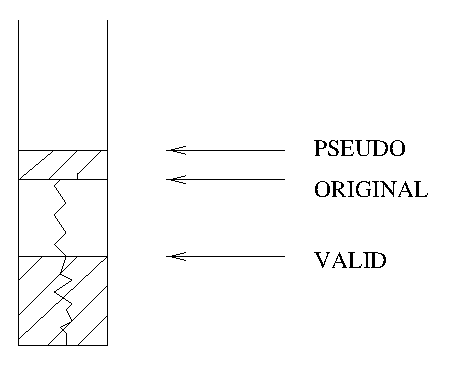
\includegraphics{Stack2.xfig.eps}}
\caption{The stack situation during the computation.}
\end{figure}
As stated the original picture $P_i$ must be protected.
The area in question is indicated by the index ORIGINAL, which
remains fixed during the lookahead computation.

The hatched area of the above illustration shows the part of the
stack which is being used in the computations at this moment. 
The area situated between ORIGINAL and PSEUDO contains a part of
stack which might have been placed in the unhatched area upwards
from VALID (thus causing the destruction of the original stack).
The special case (which in fact is the common case) when this area
between ORIGINAL and PSEUDO is empty, is perceived according to the
following illustration:(See figure 3).\\
\begin{figure}[h]
\centerline{\includegraphics{Stack3.xfig.eps}}
\caption{The area between ORIGINAL and PSEUDO is empty.}
\end{figure}
The area (in both the latter figures) below VALID is the part of
the original stack which is still in use at the moment.

We note that the index PSEUDO may both increase and decrease,
whereas VALID may only decrease.

When the lookahead routine terminates it leaves a stack situation
similar to one of the illustrations.

During the lookahead computation adequate information about the
possible sequence of reductions (mentioned above) is queued up for
use in the successor routine.

-- Successor,\\
deliveres the information about the possible reduction sequence to
the semantic interface part of the program.

On the basis of the extra information in the area on the top of the
parse stack a succeeding stack is built, resulting in the picture
$P_{i+1}$.

The transformation of the intermediate stack to the succeeding
picture may be depicted:(See figure 4).\\
\begin{figure}[h]
\centerline{\includegraphics{Stack4.xfig.eps}}
\caption{The transformation of the intermediate stack.}
\end{figure}
(The transformation of the alternative intermediate stack situation
is trivial.)
All three indices are reset to the resulting top of the stack.

- Recover,\\
transforms the picture $P_i$ into another picture $P'_k$, such 
that Lookahead $(P'_k)$ is TRUE. Recover involves the 
construction of another stack and the deletion of a number
 of input symbols. The routine is described in detail in 
the next section.

A somewhat different description of the parsing principle appiled
above is given in \cite{19}.

\subsubsection{The Recovery Algorithm}
The recovery algorithm is invoked when parsing a string not in L(G).
However, having detected an error, several possibilities of reaction
exists.
A safe but normally insufficient reaction is to stop the parsing
and inform the user about the discovered error.
A tempting reaction is to try to correct the input string, i.e. \ to
transform the erroneous input string into an error--free string.
However, in general the correction scheme is extremely complicated.
An appealing compromise is the recovery principle in which the
parser establishes a situation such that a major part of the
remaining input string may also be inspected to discover any
additional errors.
The process may involve both the restructuring of the parse stack
and the deletion of symbols from the input string.

{\em 6.2.2.1 Description of the Algorithm}\\

The recovery algorithm is activated from the parsing algorithm when
lookahead $(P_{j})$ is FALSE for some $j$. Let $P_{j}$ be\\
\begin{quote}
\begin{tabular}{|l}\hline
$t_{0} X_{1} \ldots X_{i} t_{i}$  \ \ \ \ \ \ \\ \hline
\end{tabular}
\hspace{30mm}$a_{j+1}a_{j+2} \ldots a_{n}$ \\
\end{quote}

The recovery method compiles with an outline given in \cite{18} and
works by applying error productions.
An error production has the form $A \rightarrow \alpha\;
\mbox{error}\; \beta$ where error is a special symbol.

In the algorithm the remaining input symbols are inspected one
symbol at a time.
For each symbol a sequence of stack situations is inspected, which
is constructed from the original stack by popping one stack element
at a time.
For each such stack situation the special error symbol is inserted
as the first symbol on input.
This artificial picture is now inspected.
If a successor to this picture exists, to which, furthermore,
another successor exists, then a straightforward way of recovering
from the error situation has appeared.
(Involving the described deletion of input symbols and popping of
stack elements.)

The method may be formalized in the following algorithm: (based on
$P_{j})$

\begin{tabbing}
FORi \= BEG \= BEG \= BEG \= \kill

FOR $k := j + 1$ TO $n$ DO\\
\> FOR $I := i$ DOWNTO 0 DO\\
\> BEGIN\\
\> \> LET $P^{l,k}_{error}$\\
\> \> BE 
\begin{tabular}{|l}\hline
$t_{0} X_{1}t_{1}\ldots X_{l}t_{l}$ \\ \hline
\end{tabular}
\hspace{30mm} error
$a_{k} \ldots a_{n}$\\
\> \> IF lookahead $(P^{l,k}_{error})$ THEN\\
\> \> BEGIN\\
\> \> \> $P'_{k}$ := successor $(P^{l,k}_{error})$;\\
(*) \> \> \> IF lookahead $(P'_{k})$ THEN\\
\> \> \> BEGIN\\
\> \> \> \> delete symbols $a_{j}, a_{j+1},\ldots, a_{k-1}$;\\
\> \> \> \> EXIT TO success;\\
\> \> \> END;\\
\> \> END;\\
\> END;\\
\> success: (* successful picture: $P'_{k}$ *)
\end{tabbing}

Note: A straightforward improvement of the algorithm is to extend
the check performed at ($^*$) to include 2-3 symbols instead of only a
single symbol.

{\em 6.2.2.2 Description of the Recovery Principle}\\

The detection of an error is caused by a picture $P_j$:
\begin{tabular}{|l}\hline
$t_{0} \ldots X_{i} t_{i}$ \\ \hline
\end{tabular}
\hspace{10mm} $a_{j+1} \ldots
a_{n}$, where $X_{i} = a_{j}$.\\

The existence of $P_{j}$ implies $\exists y \in \Sigma^*$ such
that
\begin{eqnarray}
 S & \Rightarrow^*_{rm} & X_{1} \ldots X_{i} y\\
& \Rightarrow^*_{rm}& a_{1} \dots a_{j}\ y \nonumber
\end{eqnarray}

The recovery method involves a specification of $k$ and $l$ $(j
< k \leq n$,$0 \leq l \leq i)$ and thereby the picture

$P^{l,k}_{error}: t_{0} \ldots X_{l} t_{l}\; \mbox{error}\;
 a_{k} \ldots a_{n}$ with the property that
 

\begin{eqnarray}
\mbox{lookahead} (P^{l,k}_{error}) &=&TRUE
\end{eqnarray}

and assuming that

\begin{eqnarray*}
P^l_k := \;\mbox{successor}\; (P^{l,k}_{\mbox{error}}) 
\end{eqnarray*}

the property that


\begin{eqnarray}
\mbox{lookahead}\; (P^l_k) &= &TRUE.
\end{eqnarray}

Inspecting the method step by a sequence of conclusions may be
stated based on the results above:

\begin{enumerate}
\item implies that for a given $l \leq i, \exists s (0 \leq s 
\leq j)$ and $\exists z \in \Sigma^*$ such that
  
    \begin{tabbing}
xxxxx \= $S$n \= $\Rightarrow^{*}_{rm}$ \=  \kill
 \>   $S$ \> $\Rightarrow^{\ast}_{rm}$ \> $X_{1} \ldots X_{l} X_{l+1} \ldots X_{i} y$\\
 \> \>   $\Rightarrow^{*}_{rm}$ \>  $X_{1} \ldots  X_{l} zy$\\
 \> \>   $\Rightarrow^{*}_{rm}$ \>  $a_{1} \ldots  a_{s} zy$
    \end{tabbing}

\item may be interpreted to mean that there exist $x =
x'' x' \in \Sigma^*, m \;(0 \leq m \leq l)$ and an error
production $A \rightarrow \alpha$  error  $\beta$ such that

        \begin{tabbing}
xxxxx \= $S$n \= $\Rightarrow^{*}_{rm}$ \= \kill
\>    $S$ \> $\Rightarrow^*_{rm}$ \> $X_1 \ldots X_m A x'$\\
 \> \>   $\Rightarrow^*_{rm} $\> $X_1 \ldots X_m
    X_{m+1} \ldots X_l\; \mbox{error}\; \beta
    x'$\\ 
\> \> $\Rightarrow^*_{rm}$ \> $X_1 \ldots X_l\;
    \mbox{error}\; x'' x'$\\
\> \> $\Rightarrow^*_{rm}$ \> $a_1 \ldots a_s \;\mbox{error} \;x$
   \end{tabbing}

where $\beta \Rightarrow^*_{rm} x''\; \mbox{and}\; \alpha =
X_{m+1} \ldots X_{l}$.

\item implies that at least one of the potential error
productions, say $A \rightarrow \beta$, is legal when the symbol
$a_k$ is included. Hence $\exists w = w''\, w' = a_k v$ such that

           \begin{tabbing}
xxxxx \= $S$\= $\Rightarrow^{\ast}_{rm}$\=  \kill
 \> $S$ \>  $\Rightarrow^{\ast}_{rm}$\> $X_{1} \ldots X_{m} A w'$\\
 \> \>  $\Rightarrow^{\ast}_{rm}$ \>  $X_{1} \ldots X_{1}\; \mbox{error}\; \beta w'$\\
 \> \> $\Rightarrow^{\ast}_{rm}$ \>  $X_{1} \ldots X_{1} \mbox{error}\, w'' w'$\\
 \> \> $\Rightarrow^{\ast}_{rm}$ \> $a_{1} \ldots a_{2} \;\mbox{error}\; a_{k} v$
     \end{tabbing}

where $\beta \Rightarrow^{\ast}_{rm} w''\;\mbox{and}\; \alpha =
X_{m+1} \ldots X_l.$
\end{enumerate}

We may now summarize the results.
The parsing algorithm has gone through the parse situations

\begin{tabular}{|l}\hline
$t_{0} X_{1} t_{1} \ldots t_{l} X_{1}$  \ \ \ \ \ \ \\ \hline
\end{tabular}
\hspace{30mm} $a_{s+1} \ldots a_{j} \ldots a_{k} \ldots a_{n}$\\
and\\
\begin{tabular}{|l}\hline
$t_{0} X_{1} t_{1} \ldots t_{l} X_{l}\ldots t_{i} X_{i}$  \ \ \ \ \ \ \\ \hline
\end{tabular}
\hspace{30mm} $a_{j+1} \ldots a_k \ldots a_{n}$\\
at which the error is detected.\\
\\
This situation is transformed into\\
\\
\begin{tabular}{|l}\hline
$t_{0} X_{1} t_{1} \ldots t_{l}X_{l}$ \\ \hline
\end{tabular}
\hspace{30mm} error $a_{k} \ldots a_{n}$\\
\\
The effect of the recovery method is to discard the symbols
$X_{l+1}\ldots X_{i}$ from the stack and to delete the
symbols $a_{j+1}\ldots a_{k-1}$ from the input string.
Recalling that

\hspace*{1cm}
$X_{l+1} \ldots X_{i}\; \Rightarrow^{\ast}_{rm}\; a_{s+1} \ldots a_{j}$

the total effect is to discard the symbol string $a_{s+1} \ldots
a_{k-1}$.
The string is replaced by the special symbol error which is part of
a string derivable from the language construct $A$.

Now the philosophy behind the recovery method may be expressed as:
While parsing the string $a_1 \ldots a_n$ an error is detected.
The error is located in the partial string $a_{s+1} \ldots
a_{k-1}$ which is supposed to reduce to a part of the language
construct $A$. 
A part of the string has been reduced into
$X_{l+1} \ldots X_{i}$ and a part remains on input. 
Both
these parts are discarded.
The succeeding picture $P'_{k}$ : 
\begin{tabular}{|l}\hline
$t_{0} \ldots X_{r} t_{r}$ \\ \hline
\end{tabular}
\hspace{30mm} $\;\;\; a_{k} \ldots a_{n}\;$\\
may be interpreted as an
element of the picture sequence evaluated from the initial picture

\hspace*{1cm}$P'_{0}:$ 
\begin{tabular}{|l}\hline
$t_{0}$ \\ \hline
\end{tabular}
\hspace{30mm} $a_{1} \ldots a_{s}\; \mbox{error}\; a_{k} \ldots a_{n}$.\\

Pictures among the successors of the picture $P'_{k}$ may cause new
error detections.
\newpage
\part{} 
\section{{\textbf Summary of terminology}}
In this section we shall give a short summary of the notion of a
context--free grammar, some parsing terminology, and an
introduction to LR--parser construction.
For a more detailed and explanatory treatment see Aho \&
Ullman [20].

Let $M$ be a set of symbols, then $M^*$ denotes the set of
{\bf all} strings of symbols from $M$, furthermore it
includes the empty string (denoted by e).

\begin{eksempel}
\mbox{}
\end{eksempel}
Let $A = \{0,1\}$, then
\begin{center}
$A^* = \{e,0,1,00,01,10,11,000,001,\ldots\}$
\end{center} 
\hfill$\Box$

\subsection{Context free grammar}

A {\bf context--free grammar} (CFG) is a 4-tuple $G =
(N,\;\Sigma,\;P,\;S)$, where
\begin{enumerate}
\item $N$ is a finite set of {\bf nonterminal symbols}.

\item $\Sigma$ is a finite set of {\bf terminal symbols}.

\item $P$ is a finite set of {\bf productions} each on the form:\\
\begin{center}
$ A \rightarrow \;\alpha$
\end{center}
where $A$ is in $N$ and $\alpha$ is in $(N \;\cup \;\Sigma)^{\ast}$.

\item $S$ is a distinguished symbol in $N$ called the
{\bf start symbol} (or goal symbol).\hfill $\Box$
\end{enumerate}


A {\bf sentential form} of a grammar $G$ is defined
recursively as follows:
\begin{enumerate}
\item $S$ is a sentential form.
\item If ${\bf \alpha} \; B \;\gamma$ is a sentential form, and $B\;
\rightarrow\; {\bf \delta}$ is a production in $P$, then
${\bf \alpha\; \delta} \;\gamma$ is a sentential form.
We say that ${\bf \alpha} \; B \;\gamma$ {\bf directly derives} 
${\bf \alpha\; \delta} \;\gamma$ and denote this by:
\begin{center}
${\bf \alpha} \;B\; \gamma \;\Rightarrow \;{\bf \alpha} \;\delta
\;\gamma$ \end{center} \hfill $\Box$
\end{enumerate}

A sentential form containing no nonterminals is called a {\bf 
sentence} generated by $G$.

The {\bf language generated by a grammar} $G$, denoted
$L(G)$, is the set of sentences generated by $G$. I.e. \ a grammar
$G$ defines a language of strings of its terminal symbols.\hfill $\Box$


We use the following conventions

\begin{tabbing}
xxxxx \= A, B, C, $\cdots$ xxxxxx\= \kill
\> $\alpha, \;\beta, \;\gamma, \;\delta, \;\ldots$ \> are in
$(N \;\cup \; \Sigma)^*$\\
\>$ a,\; b,\; c, \;d, \;\ldots$ \>  are in  $\Sigma$\\
\>$ v,\; x,\; y, \;z,\; w, \;\ldots$ \> are in $\Sigma^*$\\
\>$ A,\; B, \;C,\; \ldots$ \> are in $N$
\end{tabbing}

Let ${\bf \alpha}, \;\beta$ be sentential forms.
We say that $\alpha$ {\bf derives} $\beta$ and denote it by
$\alpha \;\Rightarrow ^*\; \beta$ if and only if:

\begin{quote}
$\alpha = \beta$ \mbox{or}\\
\mbox{there exist sentential forms}\\
$\gamma_0, \gamma_1, \ldots, \gamma_n , \;n \geq 1$
\mbox{and}\\
$ \alpha = \gamma_0, \beta = \gamma_n$, \mbox{such that}\\
$\gamma_0 \;\Rightarrow_1\gamma_n$,\\
$\gamma_1 \; \Rightarrow \;\gamma_{2}$,\\
\hspace*{5mm}$\vdots$\\
$\gamma_{n-1} \; \Rightarrow \;\gamma_n.$
\end{quote}

The sequence:
\begin{center}
$\gamma_0 \;\Rightarrow \;\gamma_1 \; \Rightarrow \;\gamma_2
\Rightarrow \;\ldots \;\gamma_{n-1} \;\Rightarrow \;\gamma_n$\\
\end{center}
is called a {\bf derivation} of $\beta$ from ${\bf \alpha}$.

A derivation is called a {\bf rightmost derivation} if, in
each step $\gamma_i \; \Rightarrow \; \gamma_{i+1}$, it is 
always the
rightmost nonterminal in $\gamma_i$ which is replaced by means of a
production. 
The symbols $\Rightarrow_{rm}\;\; \Rightarrow^*_{rm}$, indicate
rightmost derivations.

A nonterminal $E$ is called {\bf left recursive} if and
only if $E \;\Rightarrow \;\alpha \;\Rightarrow ^*\; E \;\alpha'$ for
some $\alpha,\;\alpha'$. {\bf Right recursive} is defined in a
similar way.\hfill $\Box$

A grammar $G$ is {\bf ambiguous} if and only if some sentence $w$
in $L(G)$ has more than one distinct rightmost derivation.\hfill $\Box$

\begin{eksempel}
\mbox{}
\end{eksempel}
Consider the grammar 
\begin{center}
$G_{0} = (\{E,T,P\},\{+,*,(,),a\},\cal{P},E),$
\end{center}

where $\cal{P}$ consists of\\
\begin{eqnarray*}
E & \rightarrow & E + T\\
E & \rightarrow & T\\
T & \rightarrow & T\ast P\\
T & \rightarrow & P\\
P & \rightarrow & (E)\\
P & \rightarrow & a
\end{eqnarray*}

An example of a rightmost derivation in $G_0$ is:
\begin{tabbing}
\hspace{1cm} \=  $E$n \= n$\Rightarrow_{rm}$n \= $E + T$ \= $\ast$
\=  \kill \> $E$\> $\Rightarrow_{rm}$ \>  $E + T$\\
\>\> $\Rightarrow_{rm}$ \> $E + T$ \> $\ast$ \> $P$\\
\> \>$\Rightarrow_{rm}$ \> $E + T$ \> $\ast$ \> $a$\\
\>\> $\Rightarrow_{rm}$ \> $E + P$ \> $\ast$ \> $a$\\
\>\> $\Rightarrow_{rm}$ \> $E + a$ \> $\ast$ \> $a$\\
\>\> $\Rightarrow_{rm}$ \> $T + a$ \> $\ast$ \> $a$\\
\>\> $\Rightarrow_{rm}$ \> $P + a$ \> $\ast$ \> $a$\\
\> \>$\Rightarrow_{rm}$ \> $a + a$ \> $\ast$ \> $a$
\end{tabbing} \hfill $\Box$

\subsection{Parser and parser-generator}
A {\bf parser} for a grammar $G$ is a device which, given a
string $w$ in $\Sigma^*$, checks whether this string in in $L(G)$
and, if so, outputs a possible derivation of $w$ from $S$.
Note that a string may have more than one derivation. \hfill $\Box$

A {\bf parser-generator} is a device which, given a grammar
$G$ as input, produces a parser for $G$.

In practice a parser-generator will only accept a restricted class
of grammars.
A general system would be quite inefficient and not useable for
practical purposes.
At present the biggest and most natural class of grammars for which
useable parser-generators/parsers can be constructed is the class
of LR-grammars (in particular LALR(1)).
We note that an ambiguous grammar is not an LR-grammar. \hfill $\Box$

\subsection{LR(k) grammar}
An LR-parser works by constructing a rightmost derivation backwards.
The output of the parser is the reversed sequence of productions
used in the rightmost derivation of the input string.
This reversed sequence of productions is called a {\bf right
parse}.
A sentential form is in the following always a rightmost sentential
form.

If $S \;\Rightarrow^*_{rm}\; \alpha \;A \;w \Rightarrow \;\alpha
\;\beta \;w \;\Rightarrow^*_{rm} x \;w, \mbox{where}\
x, \; w \;\in \;\Sigma^*, \mbox{then} \;\alpha \;\beta \;w$ is
a rightmost sentential form which may appear during a parse of
$x \;w$. $\beta$ is called the {\bf handle} of
$\alpha\;\beta\;w$, and $A \rightarrow \beta$ is called the {\bf
handle production}.
Given a sentential form, the purpose of the parser is to determine
the handle production.

In general the whole sentential form must be available in order to
determine the handle production.
This is not desirable in practice as the input string may be very
long.
An LR(k) grammar has the property that the handle production of
each sentential form can be uniquely determined by scanning the
sentential form from \underline{L}eft to right, producing a
\underline{R}ight parse, but only looking ahead at most
\underline{k}--symbols beyond the right end of the handle.

Let $G$ be an LR(k) grammar and let $\alpha\;\beta\;w$ be a
sentential form with handle production $A \rightarrow \beta$.
If $\alpha\;\beta\;y$ is another sentential
form, and if the first k symbols of $w$ are identical with the
first k symbols of $Y$, then $A \rightarrow \beta$ must also be
the handle production of $\alpha \; \beta \; y$.

This may be formalized in the following definitions:

{\bf Definition}\\
Let $G = (\Sigma, N, P, S),\; \mbox{and}\; \alpha \in (N \cup
\Sigma)^*$, then
\begin{center}
$FIRST_k (\alpha) = \{x \in \Sigma^* \mid \alpha 
\Rightarrow^* x w |x | = k \;\mbox{or}\;
\alpha \Rightarrow ^* x, | x | < k\}$
\end{center}
$|x|$ is the length of the string $x, |e
| = 0$ \hfill $\Box$

{\bf Definition}\\
Let $G = (N, \Sigma, P, S)$ be a CFG. Let $G' = (N \cup
\{S'\}, \Sigma, P \cup \{S' \rightarrow S\}, S')$ be its
{\bf augmented grammar}. {\bf G is LR(k)}, $k \geq 0$,
if the three conditions 
\begin{enumerate}
\item $S'\; \Rightarrow^*_{rm} \;\alpha\;  A w \;\Rightarrow\,
\alpha\; \beta \;w$, 
\item $S' \Rightarrow ^*_{rm} \gamma B x
\Rightarrow \gamma \delta x = \alpha \beta y,$ and
\item $FIRST_k (w) = FIRST_k(y)$,
\end{enumerate}

imply that $\alpha = \gamma, A = B$, and $x = y$ \hfill $\Box$

There are various technical reasons for using a new start symbol
$S'$, and a new production $S' \rightarrow S$. 
See Aho and Ullman \cite{20}.

\subsubsection{Shift--reduce parser}
In the following we shall only consider LR(1) grammars.
An LR-parser belongs to a class of parsers which all work in a
similar way.
Below we describe these parsers.

The parser uses a stack called the {\bf parse stack}.

It works as follows:\\
Initially the stack is empty and input consists of the string $w$.
\begin{tabbing}
\hspace{1cm}\= \hspace{5cm}\=\kill
            \> stack       \> input\\
            \>\begin{tabular}{|l}\hline
              \ \ \ \\ \hline
            \end{tabular}  \> $w$
\end{tabbing}

Let $w$ be divided into $x a y$ with $x, y$ in
$\Sigma^*$, and $a$ in $\Sigma$.
At a given point during the parse the $x$ part has been read
and processed and the remainder of the input is $ay$.
The parse stack will then contain a string $ \alpha$ in $(N
\cup \Sigma)^*$, such that

\[\alpha\; a \; y \; \Rightarrow ^* w\]

and such that ${\bf \alpha}\;a\;y$ is a sentential form in the right
most derivation of $w$ from $S$.
Productions used in reducing $x$ to $\alpha$ have
been outputted.
The situation is:
\begin{tabbing}
\hspace{1cm} \= \hspace{5cm} \= \kill
             \>stack         \>input \\
             \> \begin{tabular}{|l}\hline
                $\alpha$ \\ \hline
                \end{tabular}
                             \> $a y$\\
\end{tabbing}

The parser determines its next step on the basis of $\alpha$ and
$a$ (i.e. not using information about $y$).
There are four different cases:
\begin{itemize}
\item shift: read $a$ and shift in onto the stack.
\begin{tabbing}
\hspace{1cm} \=     \hspace{5cm} \= \kill
             \>stack             \>input \\
             \>\begin{tabular}{|l}\hline
               $\alpha\;a$ \\ \hline
                \end{tabular}
                                 \> $y$\\
\end{tabbing}
\item reduce: perform a reduction, that is 
$\alpha\;a\;y$ has the form 
$\gamma \delta a y$ and $B \rightarrow
\delta$ is a production and $\gamma B a y \Rightarrow_{rm} \gamma
\delta a y$ is a step in the rightmost derivation of $w$ from $S$.
The production $B \rightarrow \delta$ is outputted, and the
situation is:

\begin{tabbing}
\hspace{1cm} \= \hspace{5cm}                \= \kill
             \> stack                       \> input\\
             \> \begin{tabular}{|l}\hline
                 $\gamma\;B$ \\    
                \hline \end{tabular}
                                            \> $a\;y$\\ 
\end{tabbing}
\item accept: the stack only contains the start symbol $S$, and
input is empty.
\item error: none of the above cases is applicable; $w$ is not in
$L(G)$. \hfill $\Box$
\end{itemize}


To summarize, the parser shifts input symbols onto the stack,
until a handle appears on top of the stack. It then performs a
reduction. If no errors occur, this process is continued until the
start symbol appears on the stack. Parsers working in this way are
called {\bf shift reduce parsers}.


\begin{eksempel}
\mbox{}
\end{eksempel}

Consider a parse of the string $a + a \ast$ a in example 7.2.

\begin{tabbing}
xxxxx \= actionxxx    \=  Stackxxxxxxxxxxxxx\= Inputxxxxx  \= Output \kill 
      \> {\bf Action} \> {\bf Stack}        \> {\bf Input} \> {\bf Output}\\
\mbox{}\\
      \>              \> \begin{tabular}{|l}\hline 
                         \hspace{15mm} \\ 
                         \hline  \end{tabular}   \ \> $a + a \ast a$\\
\mbox{}\\
      \> shift        \> \begin{tabular}{|l}\hline
                         a  \\ 
                         \hline \end{tabular}   \ \> $ + a \ast a$\\
\mbox{}\\
      \> reduce       \> \begin{tabular}{|l}\hline
                         $P$   \\ 
                         \hline \end{tabular}   \ \> $+a \ast a$   \> $P \rightarrow a$\\
\mbox{}\\
    \> reduce         \> \begin{tabular}{|l}\hline
                          $T$  \\ 
                         \hline \end{tabular}  \ \> $+ a \ast a$   \> $T \rightarrow P$\\
\mbox{}\\
    \> reduce         \> \begin{tabular}{|l}\hline
                         $E$  \\ 
                         \hline \end{tabular}  \ \> $+ a \ast a$   \> $E \rightarrow T$\\
\mbox{}\\
    \> shift          \> \begin{tabular}{|l}\hline
                          $E+$  \\ 
                          \hline \end{tabular} \  \> $a \ast a$\\
\mbox{}\\
    \> shift          \> \begin{tabular}{|l}\hline
                         $E+a$  \\ 
                         \hline \end{tabular} \ \> $\ast a$\\
\mbox{}\\
   \> reduce          \> \begin{tabular}{|l}\hline
                         $E+P$  \\ 
                         \hline \end{tabular} \ \> $\ast a$        \> $P \rightarrow a$\\
\mbox{}\\
   \> reduce          \> \begin{tabular}{|l}\hline
                         $E+T$  \\ 
                         \hline \end{tabular} \ \> $\ast a$        \> $T \rightarrow P$\\
\mbox{}\\
   \> shift           \> \begin{tabular}{|l}\hline
                         $E+T \ast$  \\ 
                         \hline \end{tabular} \ \> $a$\\
\mbox{}\\
   \> shift           \> \begin{tabular}{|l}\hline
                         $E+T \ast a$  \\ 
                         \hline \end{tabular}
\\
\mbox{}\\
   \> reduce          \> \begin{tabular}{|l}\hline
                         $E+T \ast P$  \\ 
                         \hline \end{tabular} \ \>                 \> $P \rightarrow a$\\
\mbox{}\\
   \> reduce          \> \begin{tabular}{|l}\hline
                         $E+T$  \\ 
                         \hline \end{tabular} \ \>                 \> $T \rightarrow \ast \rightarrow P$\\ 
\mbox{}\\
   \> reduce          \> \begin{tabular}{|l}\hline
                         $E$  \\ 
                         \hline \end{tabular} \ \>                 \> $E \rightarrow E + T$\\
\mbox{}\\
   \> accept          \>                        \>                 \> \hspace{15mm} $\Box$
\end{tabbing}

\subsubsection{Construction of LR--parsers}
In practice the LR--parser does not just `look at' the stack and
the next input symbol to decide what to do next. The parser keeps
track of those productions which are possible candidates for a
reduction during the parse. This is done using tables, which
specify the next move at each state of the parse. These tables are
constructed by the parser generator.

Let $A \rightarrow \beta_1 \beta_2$ be a production.
Consider the derivation 
\[ S \Rightarrow ^*_{rm} \alpha ^{Aay} \Rightarrow \alpha
\beta_1 \beta_2 ay \Rightarrow ^*_{rm} \alpha \beta_1 x a y
\Rightarrow ^*_{rm} v x a y,\]
where $a \in \Sigma, y \in \Sigma^*$ or $a = e, y = e$.

During a parse of $v x a y, \alpha \beta_1$ will appear on the
stack at some stage with $x a y$ on input. When $x$ has been reduced
to $\beta_2$, then $A \rightarrow \beta_1 \beta_2$ is the handle
production and a is the next input symbol.
In general with $\alpha \beta_1$ on the stack we know nothing about
the input. But if part of the input is reduced to $\beta_2$ and a
is the next input symbol, then $A \rightarrow \beta_1 \beta_2$ is
the handle production.
The information that $A \rightarrow \beta_1 \beta_2$ is a future
candidate for a reduction when the stack contains $\alpha \beta_1$
is remembered in the following way:
\begin{quote}
\item $\alpha \beta_1$ is called a {\bf viable prefix} and we say
that $[A \rightarrow \beta_1 \cdots \beta_2, a]$
\item is an {\bf LR(1)-item} (or just LR-item) which is {\bf
valid} for $\alpha \beta_1$.
\end{quote}

In general a viable prefix has a lot of valid LR(1)-items. The set
of valid LR(1)-items for a viable prefix $\alpha \beta_1$ is
\begin{eqnarray*} 
V_1 (\alpha \beta_1)& = & \{[B \rightarrow \delta'
\cdot \delta'', b] \mid B \rightarrow\delta' \delta''\; \mbox{is a
production, and}\\
&& S \Rightarrow^*_{rm} \gamma B z \Rightarrow
\gamma \delta' \delta'' z = \alpha \beta_1 \delta'' z,\;
\mbox{and}\\
 && b \in FIRST_1 (z) \}
\end{eqnarray*} 

For a viable prefix $\alpha \;\beta_1$, $V_1(\alpha \;\beta_1)$
contains sufficient information to decide what parsing action to
take if $\alpha \beta_1$ is on the stack.

Let $\alpha \beta_1$ be on the stack, let $x$ be the next input
symbol and let $[A \rightarrow \beta_1 \ldot\ \beta_2, a]$ be in
$V_1 (\alpha \beta_1)$. There are five cases, dependent on
$\beta_2$:

\begin{enumerate}
\item $\beta_2 = x \beta_2'$.\\
I.e. \ the first symbol of $\beta_2$ is identical to the input
symbol, and the parser has to do a shift. The next state of the
parse is described by $V_1 (\alpha \beta_1 x)$, and $[A
\rightarrow \beta_1 x\ldot\  \beta'_2, a] \in V_1 (\alpha \beta_1
x)$.
\item $\beta_2 = y \beta'_2,\ y \in \Sigma, y \neq x$.\\
$A \rightarrow \beta_1 \beta_2$ is no longer a candidate for a
reduction.
\item $\beta_2 = \ B \beta'_2, B \in N$.\\
$A \rightarrow \beta_1 \beta_2$ is still a candidate for a
reduction, but we must first recognize a production of the form $B
\rightarrow \delta$. 
If and when part of the input has been reduced
to $B$, then the next state of the parse is described by $V_1
(\alpha \beta_1 B)$ and $[A \rightarrow \beta_1 B \ldot\ \beta'_2,
a] \in V_1 (\alpha \beta_1 B)$. It also follows that $\{[B
\rightarrow \ldot\ \delta, b] \mid B \rightarrow \delta$ is a
production and $b \in FIRST_1 (\beta'_2 a) \} \subseteq V_1
(\alpha \beta_1)$.
\item $\beta_2 = e$ (the empty string), $x = a.$\\
We may reduce by $A \rightarrow \beta_1$, and return the the state
$V (\alpha)$, with $\alpha$ on the stack and shift $A$ on the
stack. The next state to consider is then $V(\alpha A)$.
\item $\beta_2 = e, x \neq a$.\\
$A \rightarrow \beta_1$ is no longer a candidate for a reduction. \hfill $\Box$
\end{enumerate}


For an LR(1) -- grammar there are no conflicts between different
items of $V_1(\alpha \beta_1)$ in deciding whether to shift or
reduce.

For a non LR(1) grammar there will exist a viable prefix $\varphi$
such that $V_1(\varphi)$ contains two items of the form

\[ [A \rightarrow \beta_1 \ldots a \beta_2, b] , [B \rightarrow
\beta \ldots, a], a \in \Sigma, \]

or two different items of the form

\[ [A \rightarrow \alpha \ldots , a] , [B \rightarrow \beta
\ldots , a], a \in \Sigma \cup \{ e \}. \]

In both cases there is a conflict on the input symbol $a. V_1
(\varphi)$ is said to be {\bf inconsistent}. \hfill $\Box$

For a given set of LR-items $V_1 (\alpha)$ we define two
functions -- the {\bf parsing action function} PA, and the {\bf
successor-function} SUCC.

\subsubsection*{Definition}
Let $\alpha$ be a viable prefix of a sential form of an LR(1)
grammar $G = (N, \Sigma, P, S)$. Let $x \in \Sigma \cup
\{e\}$. 
The {\bf parsing action function}\\

\hspace*{2cm}
$PA(\vee_1 (\alpha), x)$ takes one of the values

\begin{itemize}
\item {\bf shift}, if an item $[A \rightarrow \beta_1 \ldots
x \beta_2, a] \in V_1 (\alpha)$,
\item {\bf reduce} $A \rightarrow \beta$, if an item $[A
\rightarrow \beta \ldots, x ] \in V_1 (\alpha)$,
\item {\bf accept}, if $x = e \; \mbox{and} [S' \rightarrow S
\ldots , e] \in V_1 (\alpha)$, or
\item {\bf error}, if none of the above cases are applicable. \hfill $\Box$
\end{itemize}

\subsubsection*{Definition}
Let $T - V_1 (\varphi)$ be a set of LR-items for an LR(1)
grammar $G = (N, \Sigma, P, S)$. 
Let $x \in N \cup \Sigma$.$ T' = V_1 (\varphi x) = SUCC(T, x)$ 
is the set of items computed in the following way:

\begin{enumerate}
\item The {\bf basis} of $T'$ is computed by\\
If $[A \rightarrow \alpha \ldots x \beta, a]$ is in $T$,\\
then $[A \rightarrow \alpha x \ldots \beta, a]$ is in $T'$.
\item The {\bf closure} of $T'$ is computed by
   \begin{enumerate}
    \item If $[A \rightarrow \alpha \ldots B \beta, a]$ is in
     $T'$,\\
    $B \rightarrow \delta$ is in $P$ and $b \in FIRST_1 (\beta
    a)$,\\
    then $[B \rightarrow \ldots \delta, b]$ is in $T'$.
    \item Repeat step 2.1 until no more new items can be added to
				$T'$.
     \end{enumerate}
\end{enumerate}

As there are only a finite number of LR-items for a given grammar
G, it is possible to compute in advance all the sets of LR-items
which may appear during a parse.
This is in fact done by the parser generator.

The {\bf canonical collection of sets of LR-items} may be computed
by the following algorithm.

\subsubsection*{Algorithm}
Let $G = (N, \Sigma, P, S)$ be a $CFG$. Let $G' = (N \cup \{S'\},
\Sigma, P \cup \{S' \rightarrow S\}, S')$ be the augmented grammar.
The canocical collection of sets of LR-items $\cal{A}$ is computed
by \begin{enumerate}
\item Compute the initial set $A_0$ of $\cal{A}$
   \begin{enumerate}
    \item $S' \rightarrow \ldots S, e]$ is in $A_0$
     \item Compute the closure of $A_0$
     \end{enumerate}
\item Compute the succeeding sets of $\cal{A}$
    \begin{enumerate}
     \item Let $A$ be in $\cal{A}$, and $x$ in $N \cup
\Sigma$,\\
           then compute $SUCC(A, x)$ and add it to $\cal{A}$.
     \item Repeat step 2.1 until no new set can be added to
$\cal{A}$. \hfill $\Box$
     \end{enumerate}
\end{enumerate}

A set of items in the canonical collection of LR(1)-items will in
the folowing be called an {\bf LR(1)-table} (or just an LR-table).
Note that  this term is not that used by Aho \& Ullman \cite{20}.

\subsubsection{LR-parsing algorithm}
We may now formulate the parsing algorithm using LR-tables.
Besides the symbols being stacked, the LR-tables will also be
stacked in order to find the next LR-table to be used after a
reduction.
If $PA(V_1 (\alpha \beta), a)$ is {\bf reduce} $A \rightarrow
\beta$, then $\alpha A$ will be the new stack content and $V_1
(\alpha A) = SUCC(V_1 (\alpha), A)$.

In general the stack contains\\
\begin{figure}[h]
\centerline{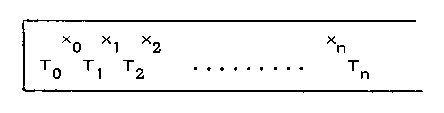
\includegraphics{Tabel2.eps}}
\end{figure}

where $T_0$ is the initial LR-table corresponding to the empty
stack and
\[ T_i = V_1 (x_1 x_2 \ldots x_i), i = 1, 2,
\ldots, n. \]

\begin{tabbing}
Algor\= be\= rep\= ca\= shiftxxxx\=beg\= xxxxx \= \ \ \ \ \=\kill
{\bf Algorithm} LR(1) parsing algorithm.\\
\> {\bf BEGIN}\\
\>  \>  \>  $T$ : = initial LR-table;\\    
\>	 \>  \>  $x$ : = next input symbol;\\
\>  \>  \>  let the stack initially contain $T$;\\
\>  \> {\bf REPEAT}\\
\>  \>  \>  {\bf CASE} $PA(T, x)$ {\bf OF}\\
\>  \>  \>  \> shift :	\> {\bf BEGIN} shift $x$ onto the stack;\\
\>  \>  \>  \>  \> \>         \> $T := SUCC(T, x)$;\\
\>  \>  \>  \>  \> \>         \> shift $T$ onto the stack;\\
\>  \>  \>  \>  \> \>         \> $x$:= next input symbol\\
\>  \>  \>  \>  \> {\bf END;}\\
\>  \>  \>  \> reduce $A \,\rightarrow \;\beta$: \> \> \> {\bf BEGIN} output $A \rightarrow \beta$;\\
\>  \>  \>  \>  \>  \> \>         \> pop 2 $\ldots | \beta |$ symbols off the stack;\\
\>  \>  \>  \>  \> \> \>          \> $T$:= LR-table on top of the stack;\\
\>  \>  \>  \>  \>  \> \>         \> shift $A$ onto the stack:\\
\>  \>  \>  \>  \>  \> \>         \> $T$:= $SUCC(T,A)$\\
\>  \>  \>  \>  \>  \>\>          \> shift $T$ onto the stack;\\
\>  \>  \>  \>  \> \>             \>{\bf END};\\
\>  \>  \>  \>  \> accept: announce accept;\\
\>  \>  \>  \>  \> error : annonce error\\
\>  \>  \>  {\bf END CASE;}\\
\>  \>  {\bf UNTIL} accept {\bf OR} error;\\
\>  {\bf END;} \hfill $\Box$
\end{tabbing}
$\Box$

\subsection{Practical LR-grammars.}
For large grammars it turns out that the size of the LR(1)-tables
and the amount of work required to construct them is very large.
However, if one considers a subset of the class of LR(1) grammars
then there exist techniques for constructing usable LR-parsers.
We shall consider two such methods.

In both methods one starts by constructing the sets of canonical
LR(0)-items (LR(0)-tables) for the given grammar.

An LR(0) table $T$ may be characterised in the following way, as a 
\begin{itemize}
\item {\bf shift table}, if $T$ contains no item of the form $[A
\rightarrow \beta \ldots , e]$,
\item {\bf reduce table}, if $T$ contains an item of the form $[A
\rightarrow \beta \ldots , e]$, and all other items have form $[B
\rightarrow \beta_1 \ldots C \beta_2, e]$.
\item {\bf inadequate table}, if $T$ contains either two items of
the form
\[ [A \rightarrow \beta_1 \ldots a \beta_2, e] , [ B \rightarrow
\cdots , e] \]
or two different items of the form
\[ [A \rightarrow \alpha \ldots , e] , [B \rightarrow \beta
\ldots , e]. \] 
\end{itemize}

The parsing action of a shift table and of a reduce table can be
determined independently of the next input symbol.
This is not the case with an inadequate table where there is more
than one parsing action which may be chosen.
Inadequate tables correspond to inconsistent sets of items in the
LR(1) case.
Consequently a grammar is LR(0) if and only if none if its
LR(0)-tables are inadequate.

In order to resolve these conflicts, each inadequate table is
converted to a {\bf lookahead table}.
An attempt could then be made to try to resolve the conflicts by
looking at the next input symbol.

Let $\alpha \beta$ be a viable prefix, let $T = V_0 (\alpha
\beta)$ be an inadequate LR(0)-table.
Let the item $[A \rightarrow \beta \ldots , e]$ be in $T$.
A lookahead set $LA(T,[A \rightarrow \beta \ldots , e]) \subseteq
\Sigma \cup \{e\}$ is computed.
The idea is that if, given a parse state described by $T$, it is
possible to reduce using the rule $A \rightarrow \beta$, then the
next input symbol will be in $LA(T,[A \rightarrow \beta
\ldots , e])$.
This can be expressed by

\begin{eqnarray*}
 LA(T,[A \rightarrow \beta \ldots e])  & \supseteq & \{a \mid
\alpha '\beta w \;\mbox{is a sentential form with} \\
V_0 (\alpha '\beta) = T, a \in  FIRST_1(w)\} 
\end{eqnarray*}

Below we describe two types of LR-grammars which differ in the way
$LA$ is defined.

Having computed $LA(T,[A \rightarrow \beta \ldots , e])$, the
item $[A \rightarrow \beta  \ldots , e]$ is replaced by $\{[A
\rightarrow \beta \ldots , a] \mid a \in LA(T,[A 
\rightarrow \beta \ldots , e]\}$. 
By doing this for all items in $T$ which may lead to a reduce, it
is possible to obtain a lookahead table $T_L$ from $T$. 
The parsing conflicts to $T$ are then resolved if the parsing
action function $PA$ can be uniquely defined on $T_L$.

There exist LR(1)-grammars for which the above way of constructing
LR-tables does not work.

\subsubsection{Simple LR(1) grammars.}
We now consider one way of defining $LA$.

\subsubsection*{Definition}
Let $T$ be an LR(0)-table.
The set of symbols for which the parsing action is shift is:
\begin{eqnarray*}
SHIFT(T) = \{ a \in \Sigma & \mid & T\; \mbox{contains an item of the form}\\
&& [A \rightarrow \beta_1 \ldots a \beta_2 , e]\}
\end{eqnarray*}  \hfill $\Box$

\subsubsection*{Definition}
Let $G = (N, \Sigma, P, S)$ be a $CFG$. Let $A \in N$, then
\[ FOLLOW_1(A) = \{ a \in \Sigma ^* \mid s \Rightarrow ^* \alpha A
w, \in FIRST_1 (w) \} \] \hfill $\Box$

\subsubsection*{Definition}
Let $G = (N, \Sigma, P, S)$ be a $CFG$.
$G$ is said to be {\bf Simple LR(1)}(SLR(1)) if any inadequate
LR(0) table satisfies the following conditions
\begin{enumerate}
\item If $[A \rightarrow \beta \ldots , e ]$ is in $T$, then
\[ FOLLOW_1(A) \cap SHIFT(T) = \emptyset\]
\item If $[A \rightarrow \alpha \ldots , e ]\; \mbox{and}\; [B
\rightarrow \beta \ldots , e ]$ is in $T$, then
\[FOLLOW_1(A) \cap FOLLOW_1(B) = \emptyset\] \hfill $\Box$
\end{enumerate}

If $[A \rightarrow \beta \ldots , e]$ is an item in an inadequate
table $T$, then $FOLLOW_1(A)$ may be used as $LA (T,[A \rightarrow
\beta \ldots , e])$.

We can define SLR(1) grammars independently of the LR(0) tables.
Let $G$ be an SLR(1) grammar, let $\alpha \beta w $ be a
sentential form with reduction handle $A \rightarrow \beta
\ldots$. If $\alpha \beta x$ is a sentential form and
$FIRST_1 (x)$ is in $FOLLOW_1(A)$, then $A  \rightarrow
 \beta$ must be the reduction handle for $\alpha \beta
 x$.

The lookahead sets of an SLR(1) grammar are not minimal.
This is because FOLLOW is computed independently of the given
inadequate state.

\subsubsection{Lookahead LR-grammars.}

We shall now consider the case with minimal lookahead sets.

If $T$ is an LR(1)-table, then we define
\[ CORE(T) = \{ [A \; \rightarrow\;  \alpha \;\ldots \;\beta, e ]
\mid [A \; \rightarrow \; \alpha \; \ldots \; \beta, a] \in T\; 
\mbox{for some} \; a\} \] 

If $T_0$ is an LR(0)-table for a grammar $G$,
then there exists an LR(1) table $T$ for $G$ such that $T_0 =
CORE(T)$, and vice versa.

\subsubsection*{Definition}

Let $G = (N, \Sigma, P, S)$ be a $CFG$.
Let $\cal{A}_0$ be the set of LR(0)-tables and let $\cal{A}_1$ be
the set of LR(1)-tables.
Let $T$ be in $\cal{A}_0$, and let $T$ contain an item of the form
$[A \rightarrow  \beta \ldots , e]$.
We define 
\begin{eqnarray*}
 LALR_1(T,[A \rightarrow \beta \ldots , e]) = \{a \in \Sigma &
\mid & [A\;  \rightarrow \beta \ldots , a] \in T', T' \in 
\cal{A}_1, \\
&&\mbox{and}\; CORE(T') = T\}
\end{eqnarray*}
\hfill $\Box$

\subsubsection*{Definition}
Let $G = (N, \Sigma, P, S)$ be a $CFG$.
$G$ is said to be {\bf Lookahead LR(1)} (LALR(1)) if any inadequate
table $T$ satisfies the following conditions:

\begin{enumerate}
\item If $[A \; \rightarrow \; \beta \,\ldots , e] \in T$, then\\
$LALR_1(T,\{T,[A \;\rightarrow \;\beta \,\ldots , e]) \; \cap
SHIFT(T) = \emptyset$
\item If $[A \;\rightarrow \;\alpha \;\ldots , e] \;\mbox{and}/; [B
\; \rightarrow \,\beta \;\ldots , e] \in T$, then\\
$LALR_1(T,[A \;\rightarrow \;\alpha \,\ldots , e]) \;\cap
\; LALR_1(T,[B \;\rightarrow \,\beta \,\ldots , e]) = \emptyset$ \hfill $\Box$
\end{enumerate}


The lookahead sets $LALR_1(T,[A \rightarrow \beta \ldots , e])$
can be computed directly from the LR(0)-tables without computing
the LR(1)-tables.
An algorithm for doing this is given in [23].

It may be difficult for an unexperienced reader to distinguish
between the various types of grammars.

In practice the following rules seem to apply:

\begin{itemize}
\item It often happens that an LR(1) grammar which is not SLR(1) is
LALR(1).
\item It is not very common that a grammar which is not LALR(1) is
in fact LR(1).
Usually such a grammar is ambiguous.
\end{itemize}

We end this section with an example of an LALR(1) grammar which is
not SLR(1).

\subsubsection*{{\bf Example}}
Consider the grammar $G = (\{S', S, A\},\{a, b, c,  d, f\}, P, S')$
where $P$ consists of

\begin{tabbing}
\hspace*{3cm} \= $S'$ xx \= $\rightarrow$ \= xx \kill
\> $S'$\> $\rightarrow$ \> $S$\\
\> $S$ \> $\rightarrow$ \> $aAd$\\
\> $S$ \> $\rightarrow$ \> $afc$\\
\> $S$ \> $\rightarrow$ \> $bAc$\\
\> $S$ \> $\rightarrow$ \> $bfd$\\
\> $A$ \> $\rightarrow$ \> $f$
\end{tabbing}

The LR(0) tables for $G$ are ($\rightarrow$ indicates the $SUCC$ function) 
\newpage

\begin{figure}[h]
\centerline{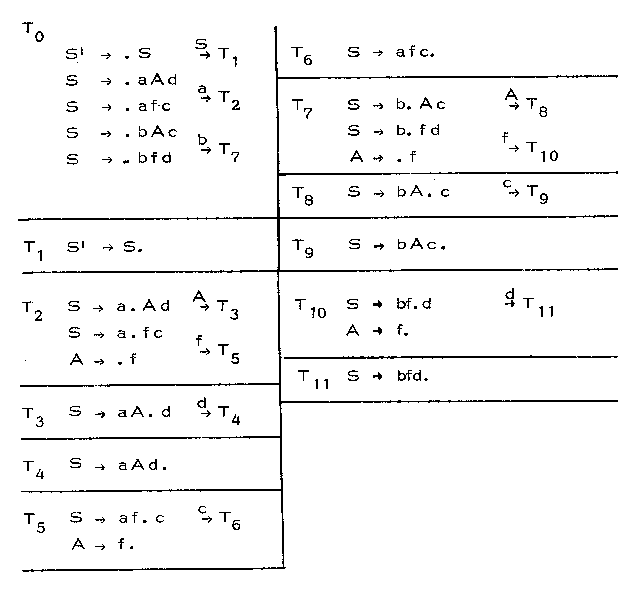
\includegraphics{Tabel.eps}}
\caption{The gramma G}
\end{figure}

\begin{tabbing}
$G$ is not $LR(0)$ since $T_{5}$ and $T_{0}$ are inadequate.\\
$G$ is not $SLR(1)$ since $FOLLOW_{1}(A) = \{ c,d \}$.\\
$G$ is $LALR(1)$ \= since $LALR_{1}(T_{5}, [A \rightarrow f \ldot, e]) = \{d\}$\\
                 \> and $LALR_{1}(T_{10}, [A \rightarrow f \ldot, e]) = \{c\}$
\end{tabbing}
\newpage

\begin{thebibliography}{99}

\bibitem[1]{1}
DeRemer, F.L.,\\
\textit{Practical Translation for LR(K) Languages},\\
Ph.D. Thesis, Massachusetts Inatitute of Technology,\\
Cambridge(Mass), Okt. 1969

\bibitem[2]{2}
DeRemer, F.L.\\
\textit{Simple LR(k) grammars}\\
Comm. ACM 14, 453 - 460 (1971)

\bibitem[3]{3}
Knuth, D.E.\\
\textit{On the translation of languages from left to right}\\
Information and Control 8, 607 - 639 (1965)

\bibitem[4]{4}
Lalonde, W.R.\\
\textit{An Efficient LALR-Parser-Generator}\\
Tech. Report CSRG-2, University of Toronto\\
Toronto, Ontario, 1970

\bibitem[5]{5}
Horning J.J. and Lalonde, W.R.\\
\textit{Empirical Comparison of LR(k) and precedence Parsers}\\
Toronto, Ontario, 1970

\bibitem[6]{6}
Wirth, N.\\
\textit{The programming Language Pascal}\\
Acta Informatica, 1, 35 - 63 (1971)

\bibitem[7]{7}
Jensen, B.B., Madsen, O.L., Kristensen, B.B. and Eriksen, S.H.\\
\textit{BOBS-System Brugervejledning}\\
DAIMI PB-10 (in Danish), March 1973\\
DAIMI, University of Aarhus

\bibitem[8]{8}
Kristensen, B.B., Madsen, O.L., Jensen B.B., and Eriksen, S.H.\\
\textit{A Short Description of a Translator Writing system (BOBS-System)}\\
DAIMI PB-11, February 1973\\
DAIMI, University of Aarhus

\bibitem[9]{9}
Kristensen, B.B, Madsen, O.L., Jensen B.B., and Eriksen, S.H.\\
\textit{BOBS-system. Tilf{\o}jelser og {\ae}ndringer til brugervejledning}
DAIMI PB-22 (in Danish), January 1974\\
DAIMI, University of Aarhus

\bibitem[10]{10}
Kristensen, B.B, Madsen, O.L., Jensen B.B., and Eriksen, S.H.\\
\textit{A Short Description of a Translator Writing System (BOBS-System)}
DAIMI PB-41, October 1974\\
DAIMI, University of Aarhus

\bibitem[11]{11}
Burger, W.F.\\
\textit{BOBSW - A Parser Generator}\\
SESL TR-7, december 1974\\
Department of computer Science\\
The University of Texas At Austin

\bibitem[12]{12}
Jensen, K. and Wirth, N.\\
\textit{Pascal User Manual and Report}\\
Springer Verlag, 1975

\bibitem[13]{13}
Kristensen, B.B, Madsen, O.L. and Jensen B.B.\\
\textit{An Implementation of a Pascal Compiler}\\
Unpublished paper, April 1974\\
DAIMI, University of Aarhus

\bibitem[14]{14}
Kristensen, B.B.\\
\textit{Erkendelse og korrektion af syntax fejl under LR-parsing}\\
Master Thesis (in Danish), May 1974\\
DAIMI, University of Aarhus

\bibitem[15]{15}
Jensen, B.B.\\
\textit{An Extension of the BOBS-System to a full Compiler-Compiler Based om Mathematical Semantics}\\
Master Thesis, February 1975\\
DAIMI, University of Aarhus

\bibitem[16]{16}
Mosses, P.\\
\textit{The Mathematical Semantics and Compiler Generation}\\
Ph.D. Thesis, September 1974\\
Oxford University Programming Research Group\\
Oxford, England

\bibitem[17]{17}
Madsen, O.L.\\
\textit{On the Use of Attribute Grammars in a Practical Translator Writing System}\\
Masters Thesis, July 1975\\
DAIMI, University of Aarhus

\bibitem[18]{18}
Aho, A.V. and Johnson, S.C.\\
\textit{LR-Parsing}\\
Computing surveys 6, 99 - 124 (June 1974)

\bibitem[19]{19}
Eve, J.\\
\textit{On the Recovery of LR(1) Parsers from computed Parsing Tables}\\
Computing Laboratory\\
The University of Newcastle upon Tyne\\
England

\bibitem[20]{20}
Aho, A.V. and Ullman, J.D.\\
\textit{The Theory of Parsing, Translation and Compiling}\\
Volume 1: Parsing, 1972\\
Volume 2: Compiling, 1973\\
Prentice Hall, Englewood Cliffs (N.J.)

\bibitem[21]{21}
Knuth, D.E.\\
\textit{Semantics of context Free Languages}\\
Mathematical systems Theory, vol. 2 (1968) 127 - 145

\bibitem[22]{22}
Lewis, P.M., Rosenkrantz, D.J. and Stearns, R.E.\\
\textit{Attribute Translation}\\
Journal of Computer and System Sciences 9, 279 - 307 (1974)

\bibitem[23]{23}
Kristensen, B.B., Madsen, O.L.\\
\textit{Methods for computing LALR(k) Lookahead}\\
ACM Transactions on Programming Languages 3, 60 - 82 (1981)

\end{thebibliography}

\end{document}




 

































